%%%%%%%%%%%%%%%%%%%%%%%%%%%%%%%%%%%%%%%%%%%%%%%%%%%%%%%%%%%%%%%%%%%%%%
%     File: ExtendedAbstract_imple.tex                               %
%     Tex Master: ExtendedAbstract.tex                               %
%                                                                    %
%     Author: Andre Calado Marta                                     %
%     Last modified : 27 Dez 2011                                    %
%%%%%%%%%%%%%%%%%%%%%%%%%%%%%%%%%%%%%%%%%%%%%%%%%%%%%%%%%%%%%%%%%%%%%%
% A Calculation section represents a practical development
% from a theoretical basis.
%%%%%%%%%%%%%%%%%%%%%%%%%%%%%%%%%%%%%%%%%%%%%%%%%%%%%%%%%%%%%%%%%%%%%%

\section{Results}
\label{sec:imple}
\vspace{0.2cm}
\subsection{Stabilization}
Determinant Quantum Monte Carlo suffers from low temperature and large size numerical instabilities.
These arise because the information about the quantum states we seek is encoded in the differences between matrix elements of largely different magnitude contained in the elements of the $\bm B$-matrices of Eq.(\ref{eq:Z_quadratic}).
It is outside of the scope of this document to describe the stabilization procedure (it is done in the thesis).
In short, we find the energy scales that gives us the relevant information we seek via a $\bm Q \bm R$ decomposition with partial pivoting (following \cite{bai_stable_2011}), and then we cut off the irrelevant scales that destabilize the matrix products we need to compute, using a matrix $\bm D'$ (the notation becomes clear in the thesis).
\begin{figure}[H]
  \centering
  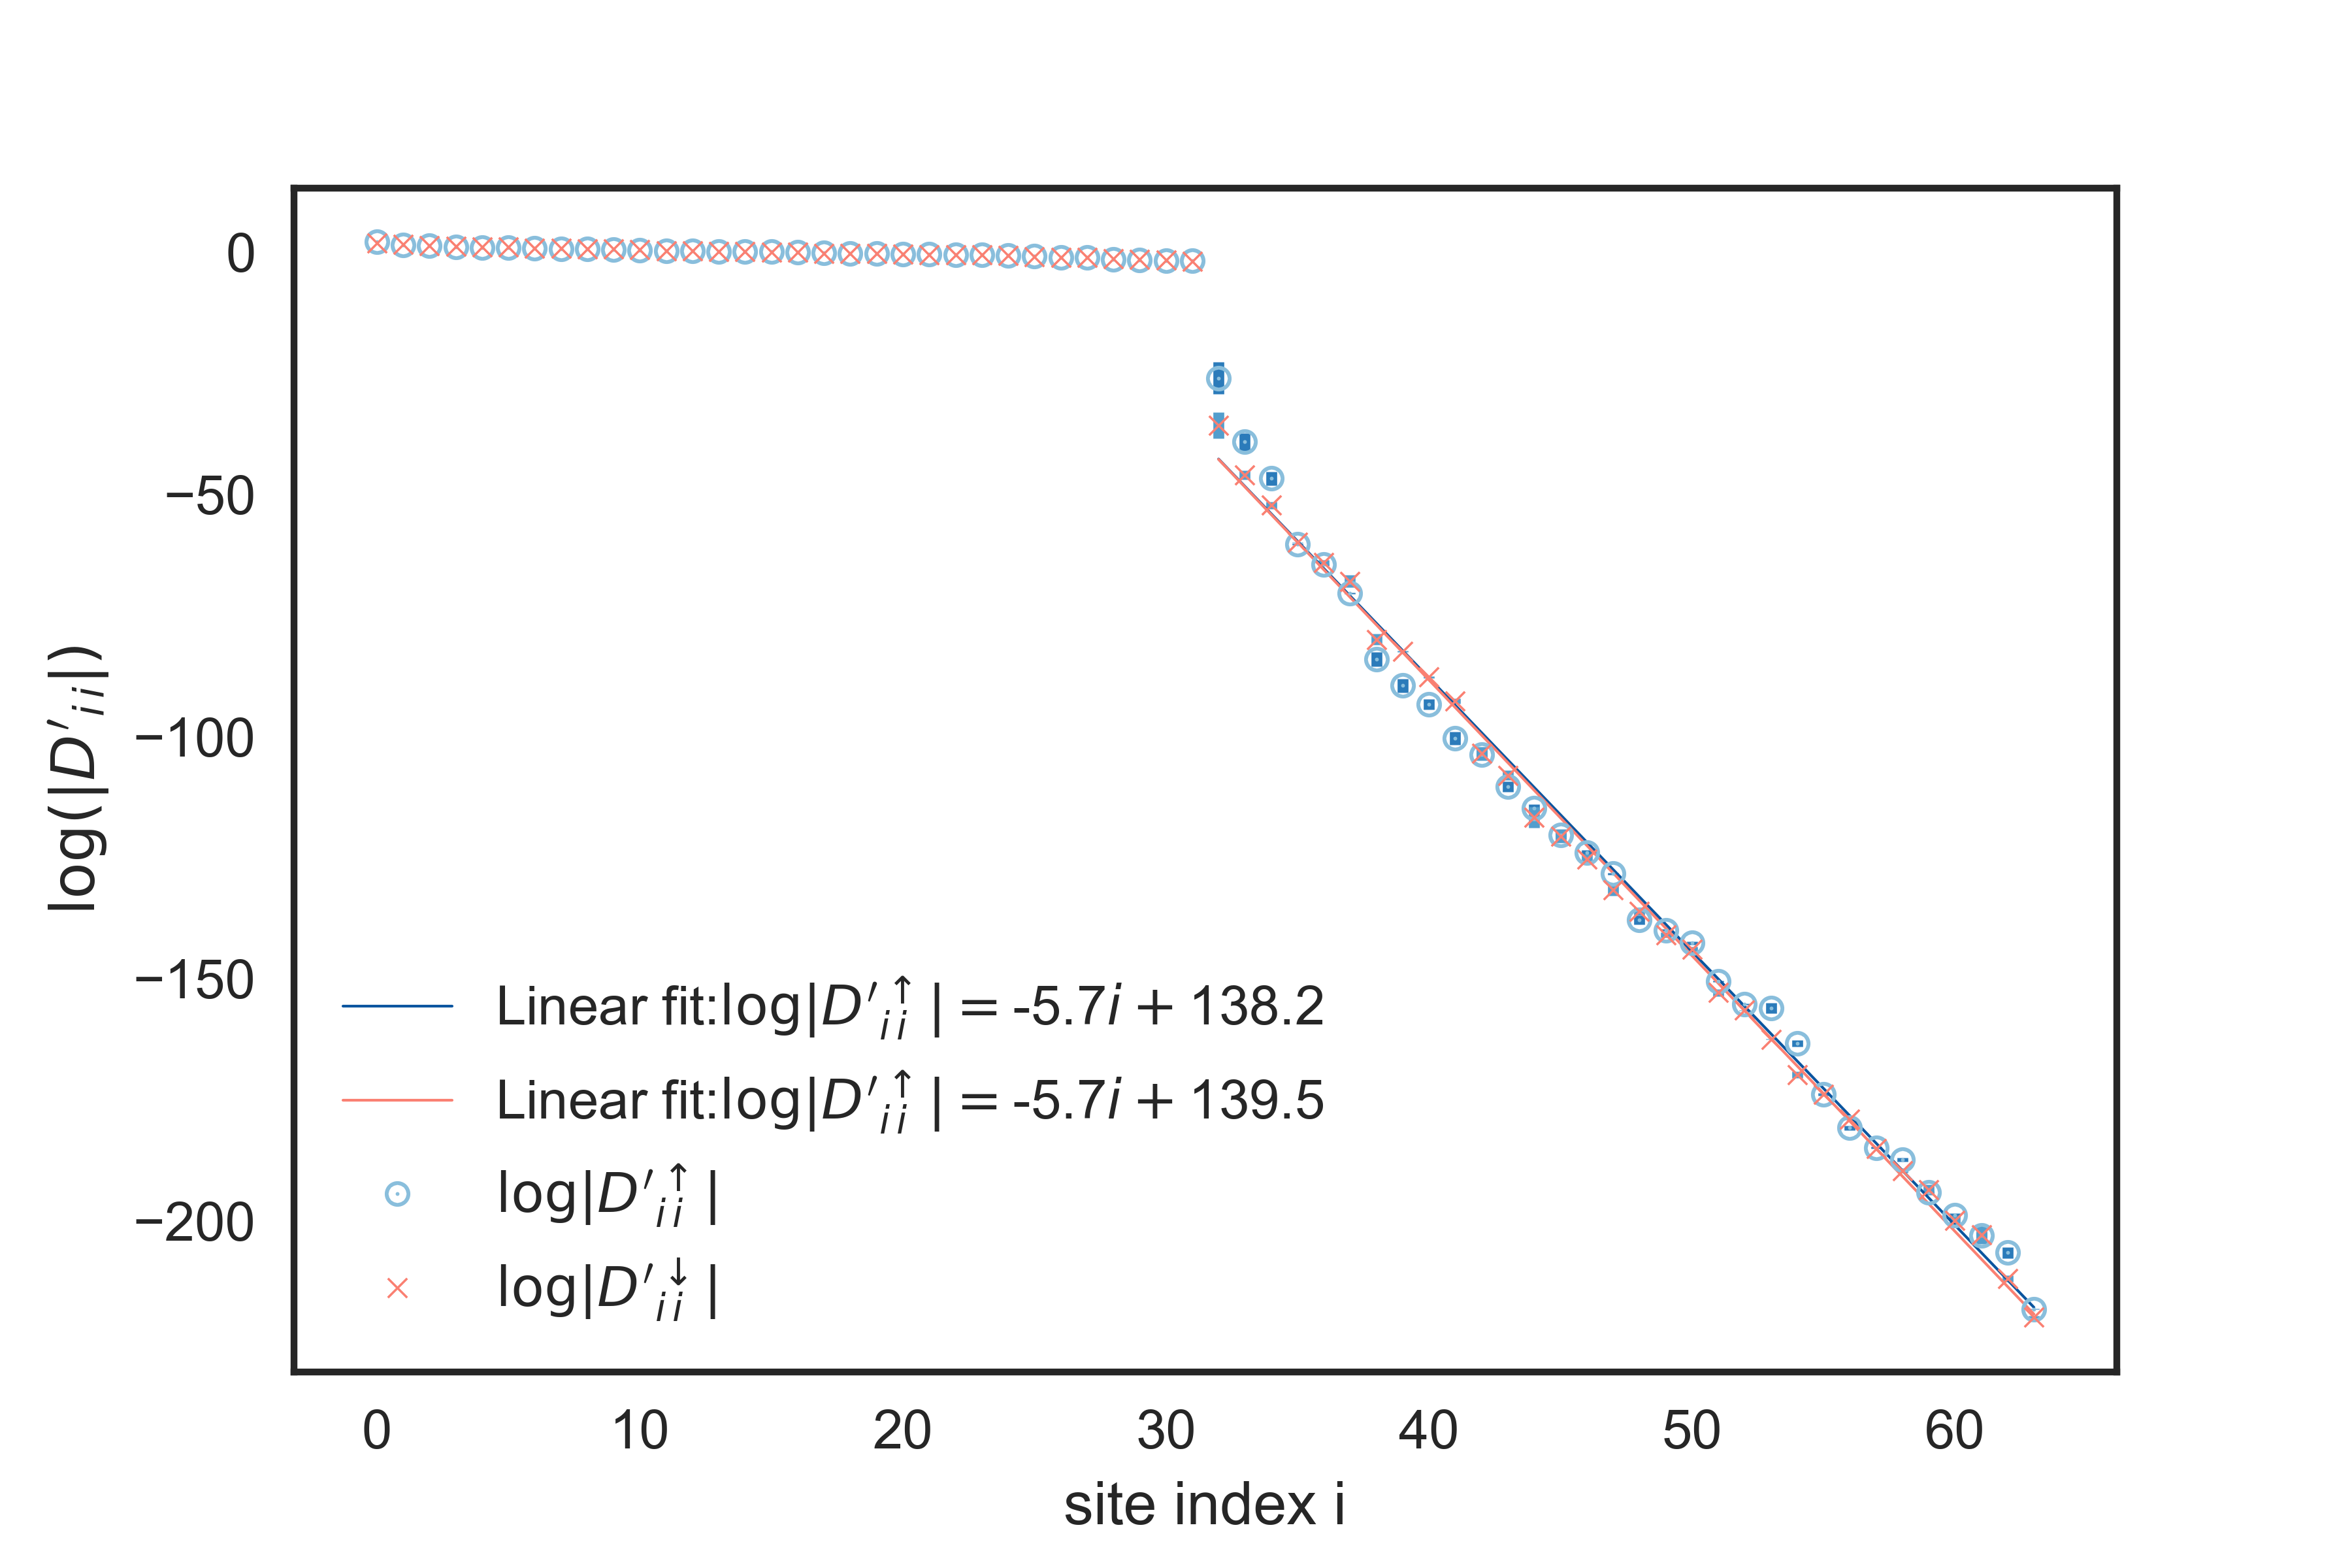
\includegraphics[width =7.5cm]{images/OrdersOfMagnitude_N=64sites.png}
  \caption{The matrix $\bm D'$ (standard notation used in the thesis) displays the scales spanned by the stably multiplied $\bm B$-matrices (in this case for $\beta = 20t$, $U = 8t$, on a 64-site 1D chain with periodic boundary conditions).}
  \label{fig:numerical_scales}
\end{figure}
\subsection{Benchmarks}
Our comparison with the auxiliary field QMC results of \texttt{QUEST} for a 64-site 1D chain with periodic boundary conditions with $U = 4 t$, and $\beta = 25 t$, shows remarkable agreement, namely in the magnetic structure factor.
\begin{figure}[H]
  \centering
  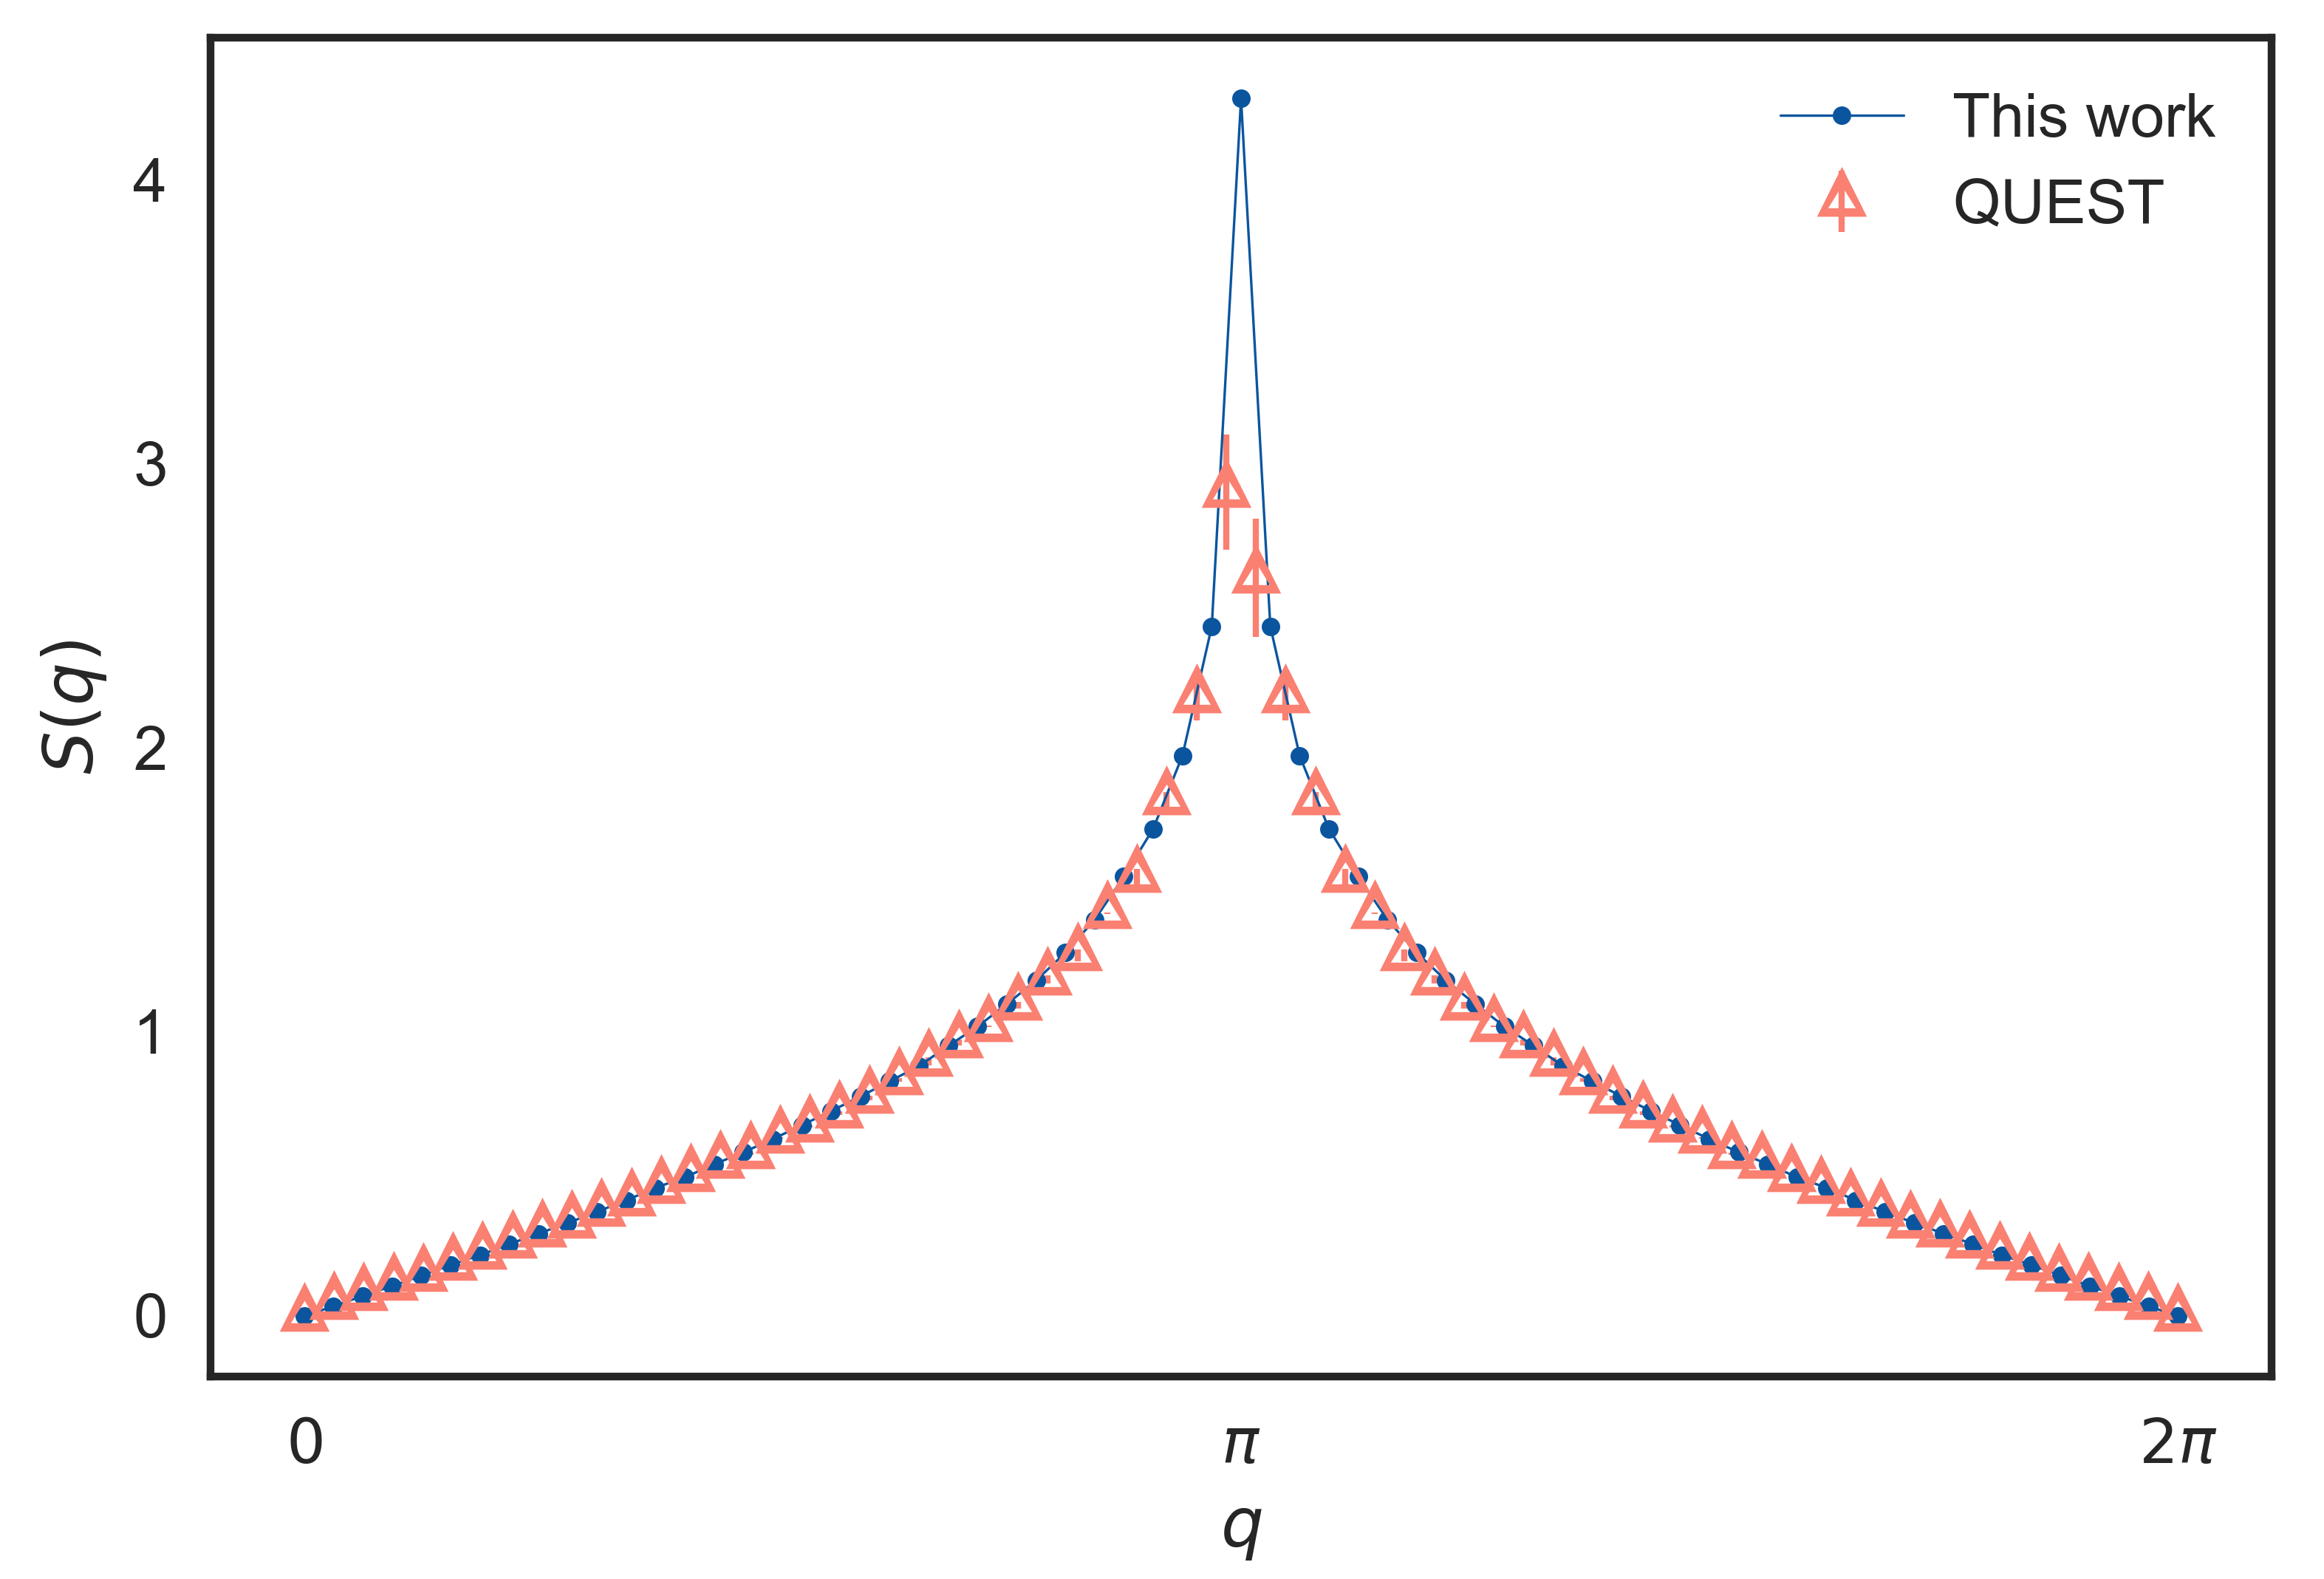
\includegraphics[width=7.3cm]{images/s_compare.png}
  \caption{Comparison between our measurement of the magnetic structure factor and the result obtained when we ran \texttt{QUEST}}
  \label{figdetVSquest}
\end{figure}
Another benchmark is the result that we obtain for the magnetic ordering in a strained graphene nanoribbon, reproducing the results of a recent paper \cite{yang_strain-tuning_2017}.
The prediction of our mean field calculation for a strained graphene nanoribbon (with hoppings reduced along its longitudinal $x$ direction $t \mapsto t - \Delta, \Delta = 0.3t$) is that the spins along the rows of the ribbon have uniform correlation.
In fact, we can see that mean field overestimates long range ordering, and they follow instead the symmetric profile of Fig.(\ref{fig:corrProf}), a behavior typical of this type of graphene-based system \cite{feldner_dynamical_2011, raczkowski_interplay_2017}.
This result expands on the study carried out in \cite{yang_strain-tuning_2017}.
\begin{figure}[H]
  \centering
  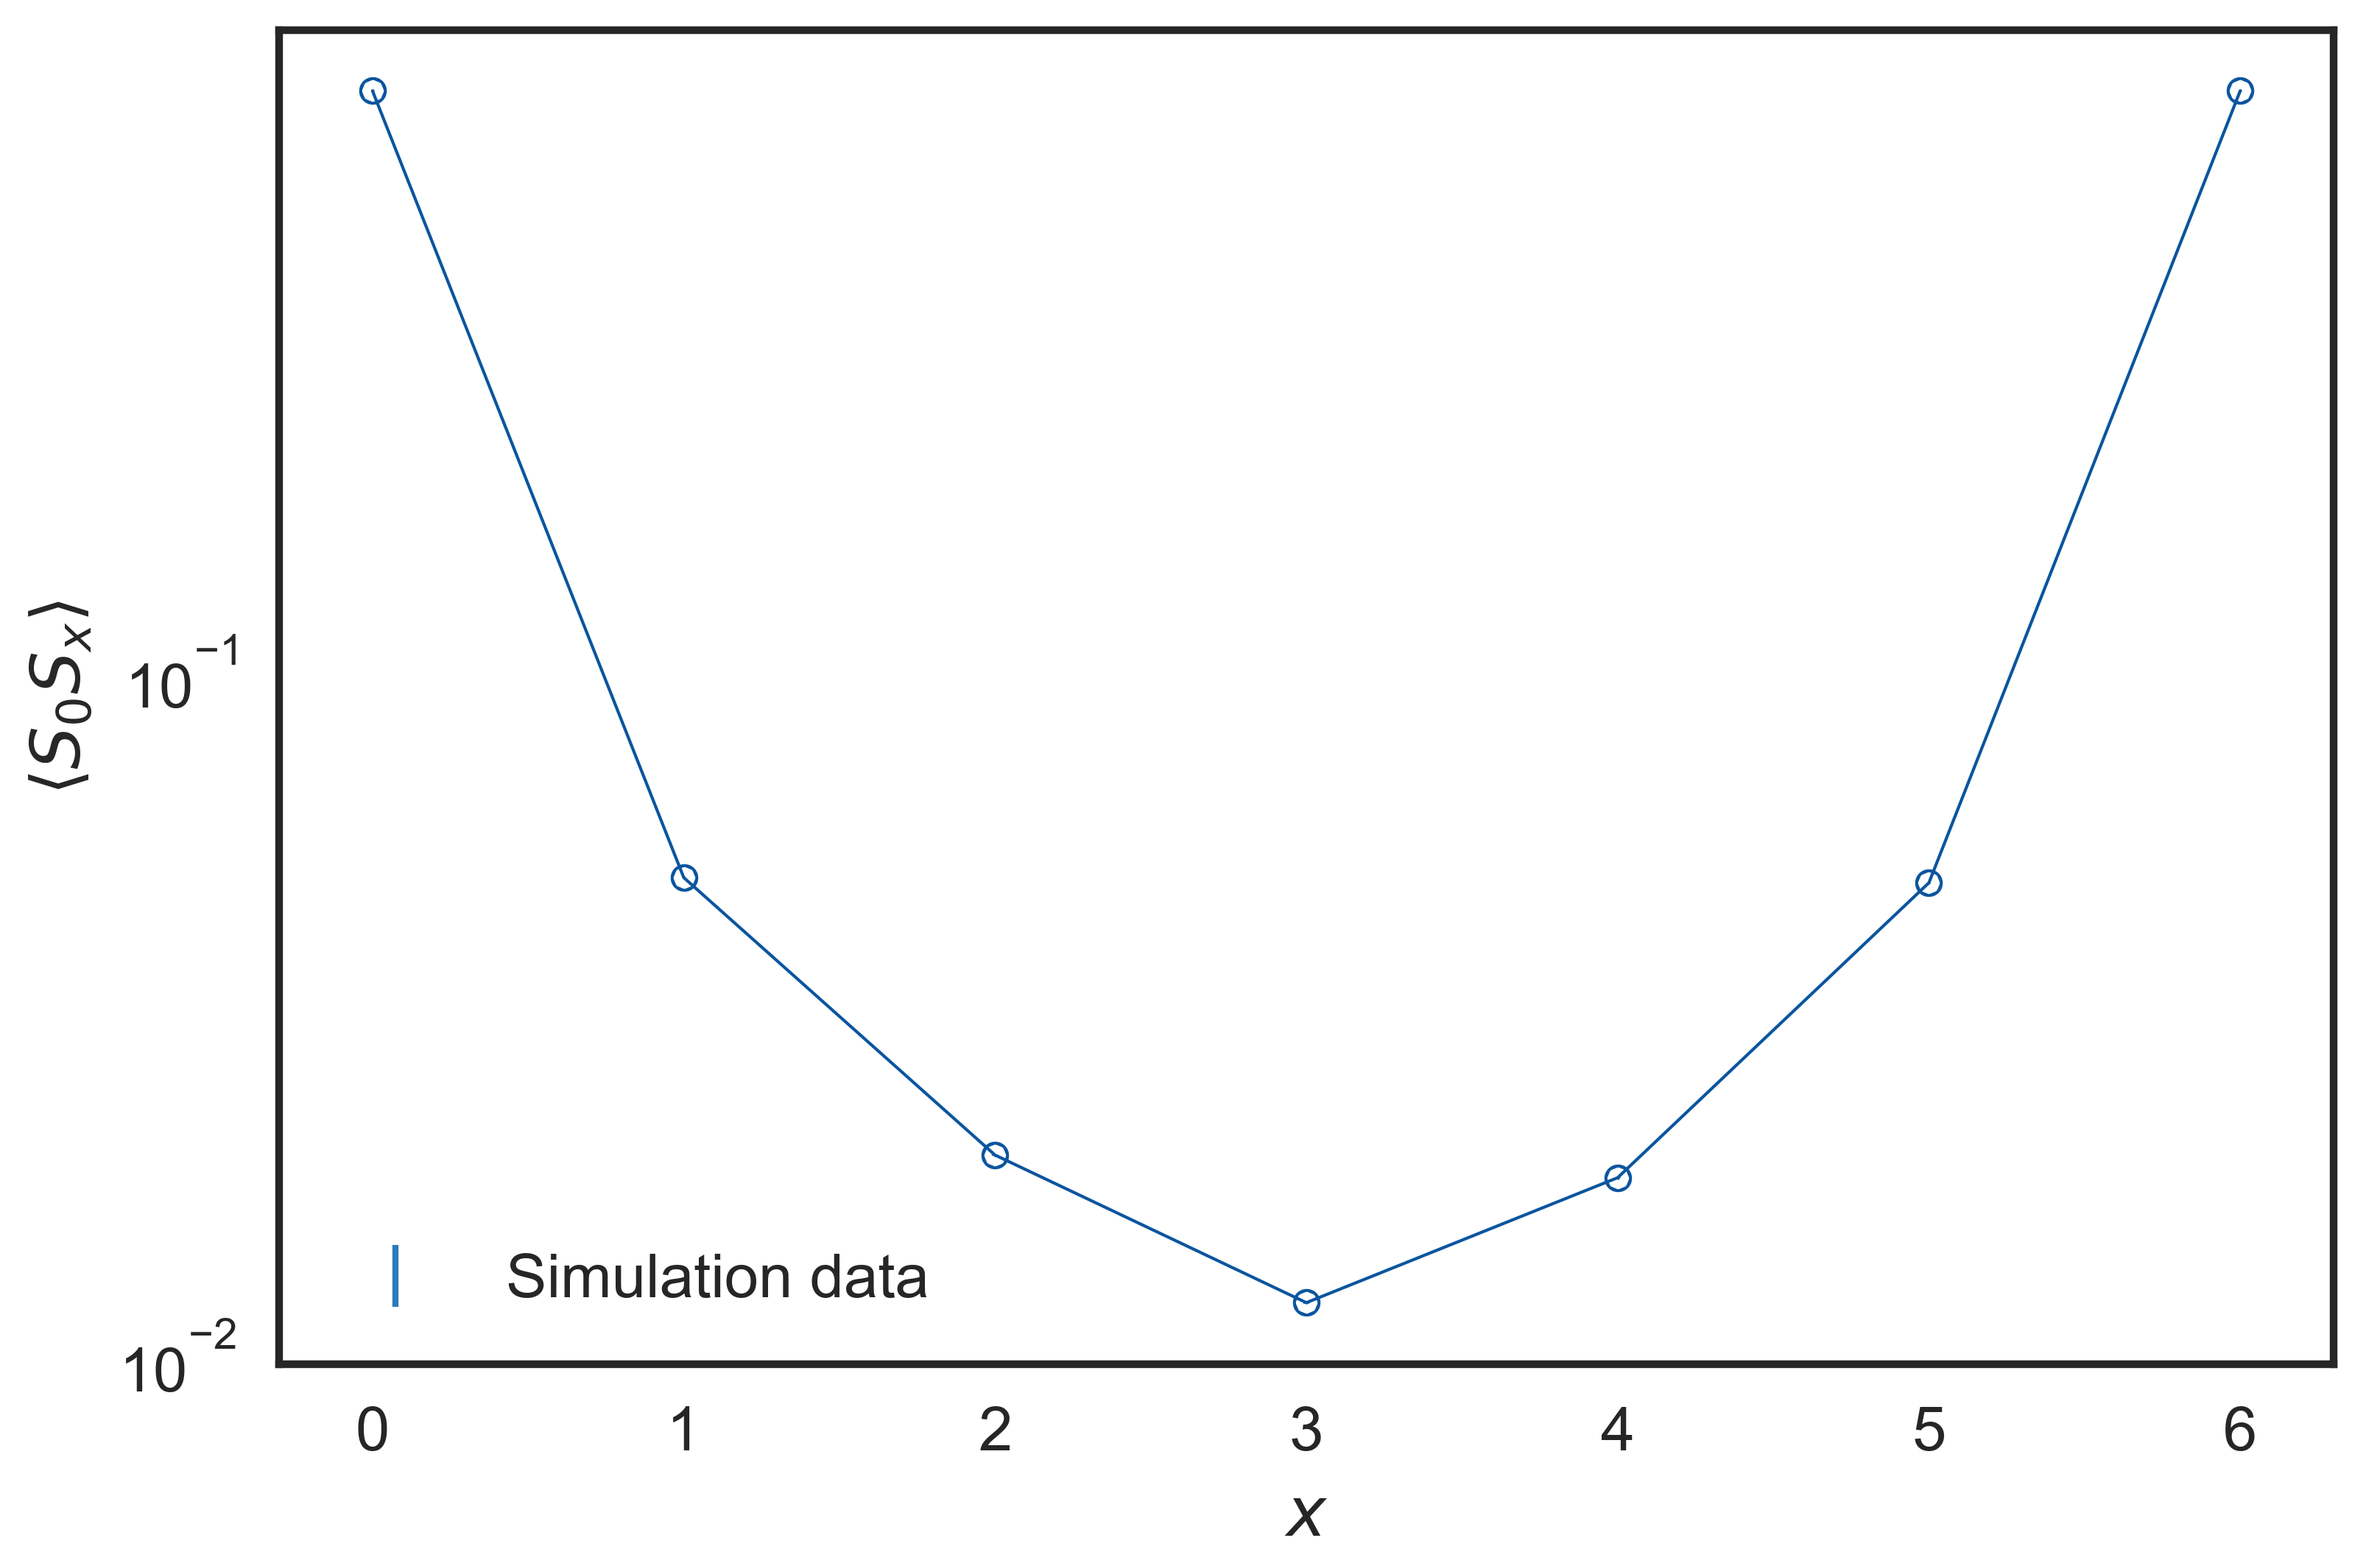
\includegraphics[width = 7.5cm]{images/LongitudinalProfile.png}
  \caption{Profile of the spin-spin correlations along the edge for a $ 6 \times 6$ strained graphene nanoribbon at $\beta = 16$, $U = 3t$, $\Delta = 0.3$.}
  \label{fig:corrProf}
\end{figure}
By computing the susceptibility on the edge (restricting the sum in Eq.(\ref{eq:chi}) to sites on the edge) for one of the sublattices, we are to find the critical temperature for the transition to the ordered state for $U = 3 t$, $T_c = ( 0.017 \pm 0.003 ) t$.
This is done by fitting the results for the susceptibility obtained for our simulates run at different temperatures to the Curie Law $\chi \propto ( T - T_c )^{-1}$ (see Fig.(\ref{fig:chiFit}).
Repeating the procedure for varying temperature, and on-site interaction, we would be able to draw a complete phase diagram.
\begin{figure}[H]
  \centering
  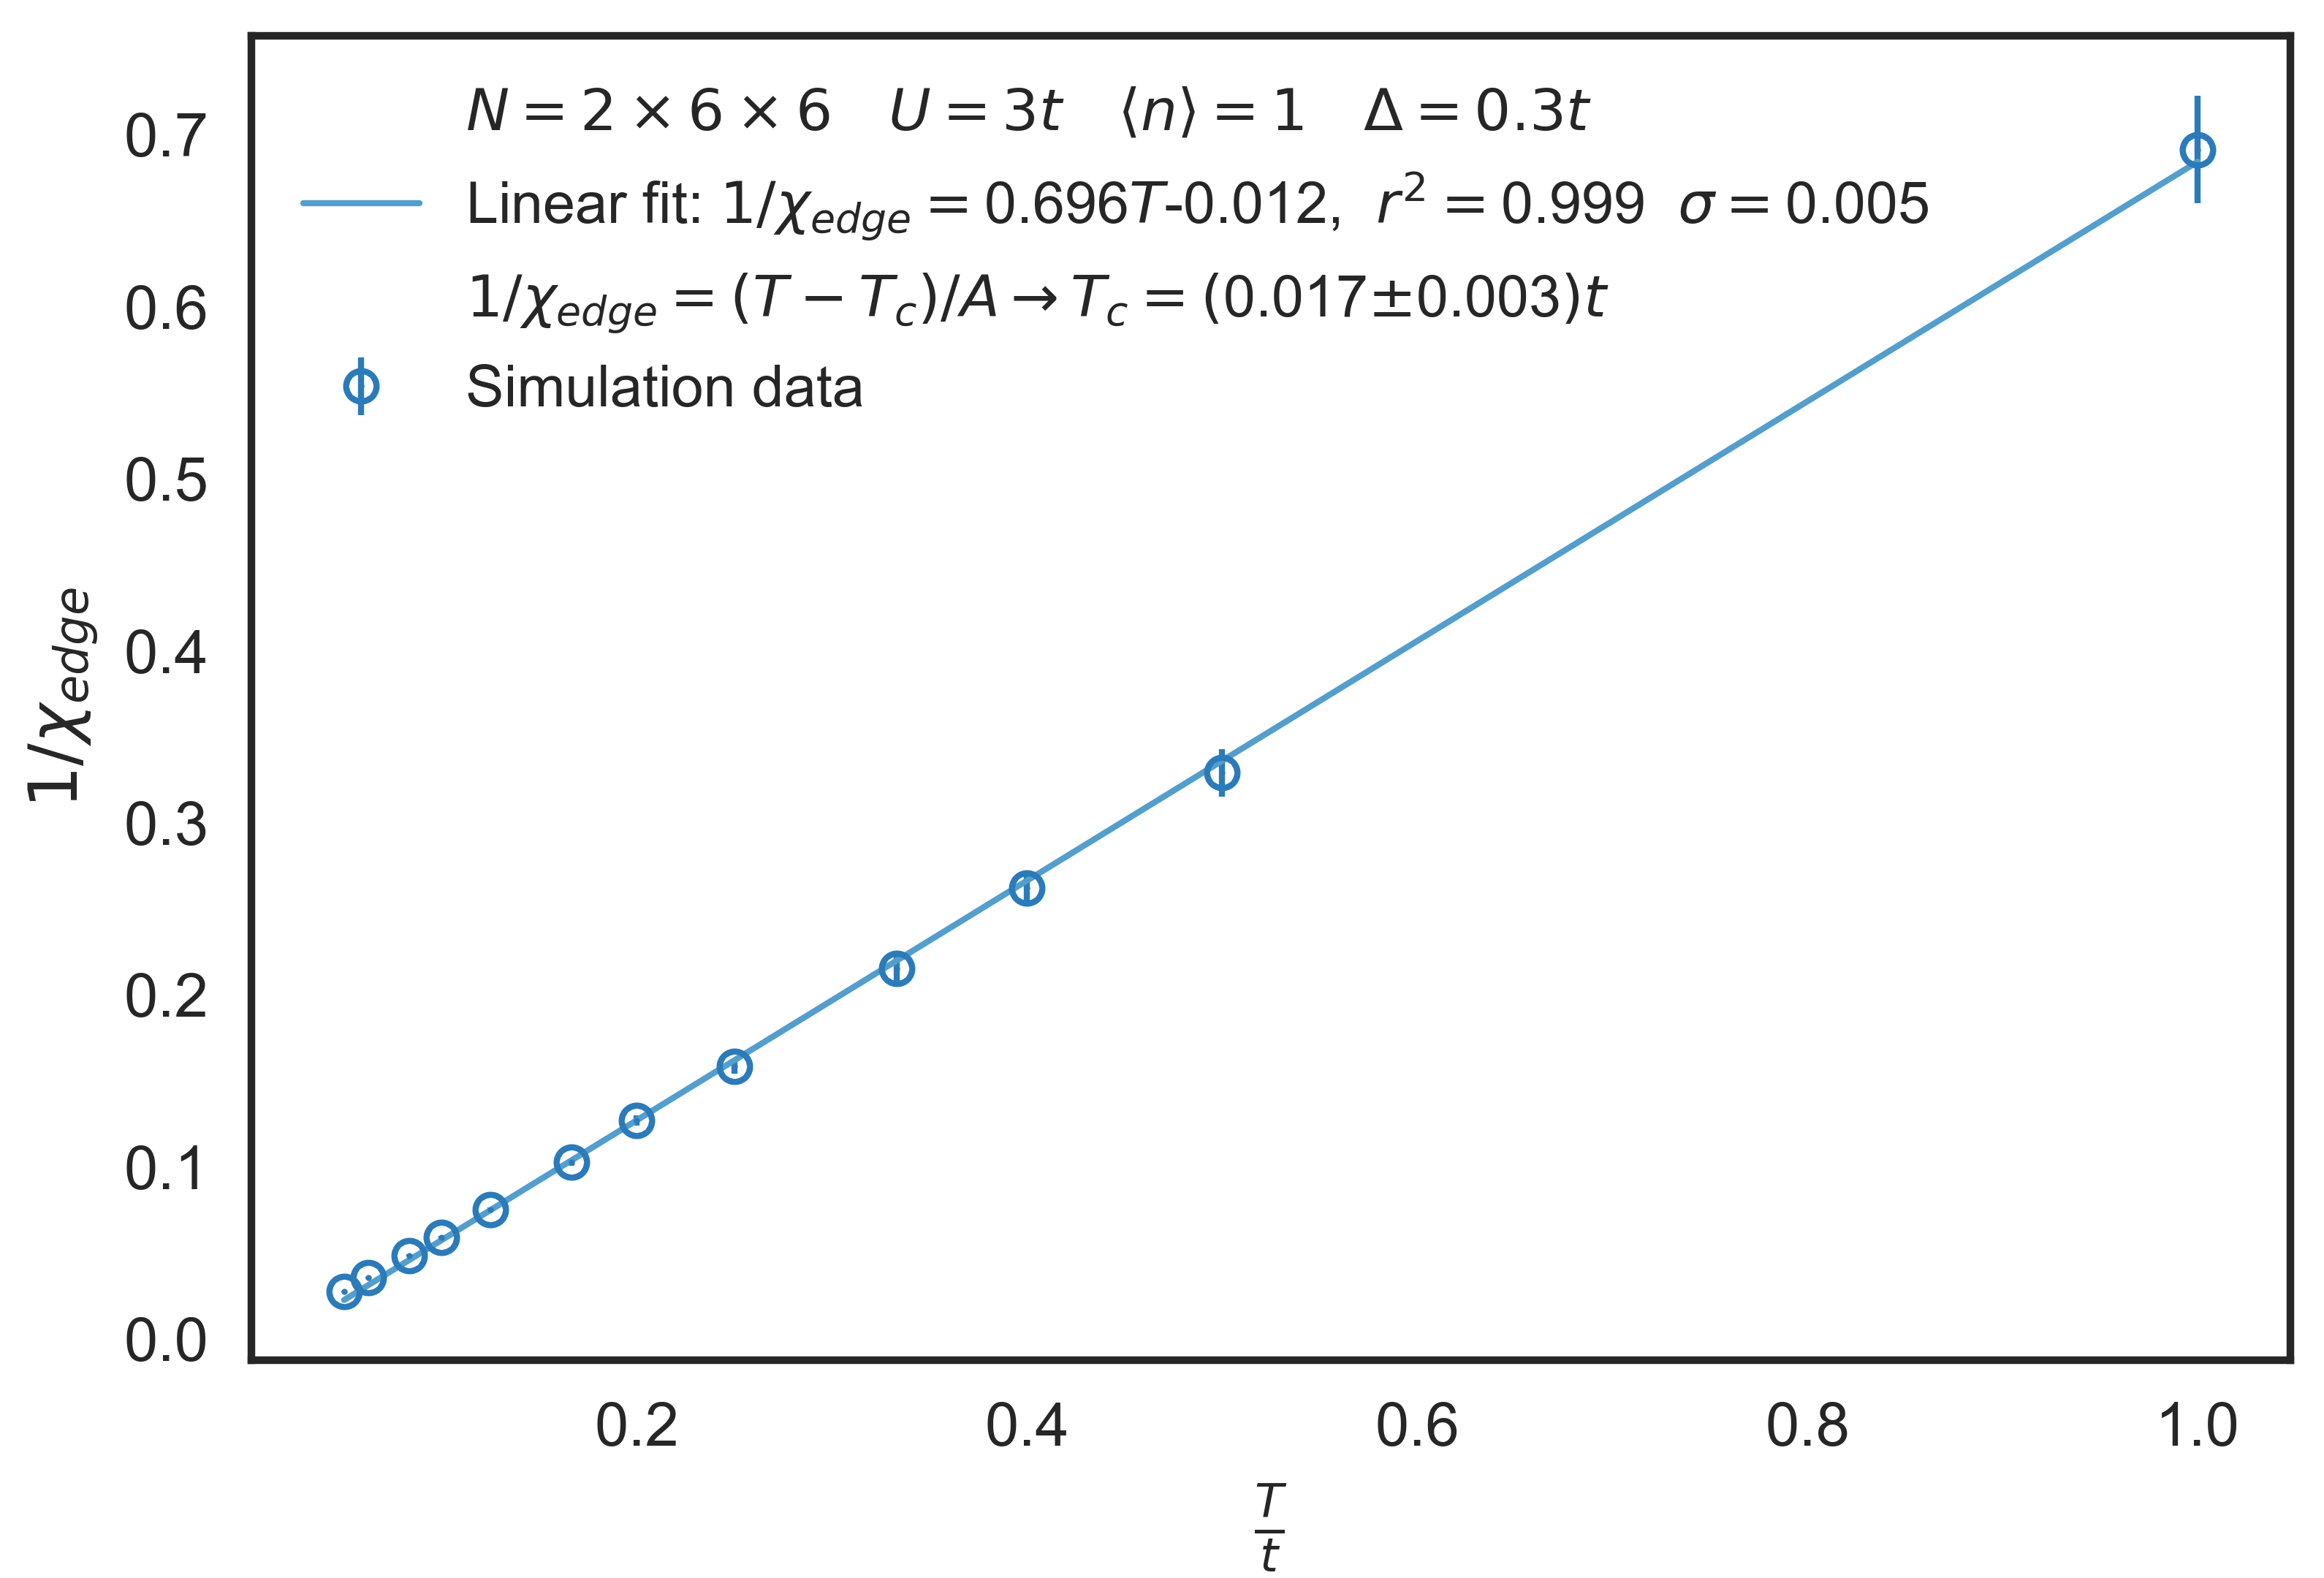
\includegraphics[width=7.3cm]{images/fityang2017.png}
  \caption{Fit of $\chi_{\text{edge}}$ to Curie's Law.}
  \label{fig:chiFit}
\end{figure}

\subsection{Mean field}
\label{sec:resul}
In Fig.(\ref{fig:nanoGraphVsTMD}), we compare the magnetization profile along the rows of the ribbon ($y$ is the transverse coordinate) for a graphene nanoribbon with the homologous profile obtained for a TMD nanoribbon, within the ordered phase.

In Fig.(\ref{fig:bandsU20}), we present the spin-resolved band structure within the ordered phase of a TMD nanoribbon of width $N_y = 16$.
The first two aspects to notice are that spin degeneracy has been lifted, and that the shape of the bands has been distorted.
The part of the bands near the Fermi energy $\varepsilon_F$ determines the physics of the phase.
The interplay between the geometry of the tight-binding model, its parameters, the on-site interaction and temperature gives rise to different phases since it determines the shape of the bands and the location of the Fermi energy corresponding to charge neutrality.
Two changes with respect to the free bands are crucial:
the K-point splitting (circled in yellow), corresponding to a region where one of the bands stays below the Fermi energy, while the other stays above - this leads to spin polarization of the eigenstates associated with these energies; the band crossing (circled in green) - as $U$ varies, and the bands move upward or downward, and eventually distort, the states around this band crossing become either occupied or unoccupied.
This will lead to the appearance of a magnetization with a magnitude that depends on the specific point in $k$ where the two bands meet, once the intersection point is related to which states are occupied or unoccupied.
\begin{figure}[H]
\centering
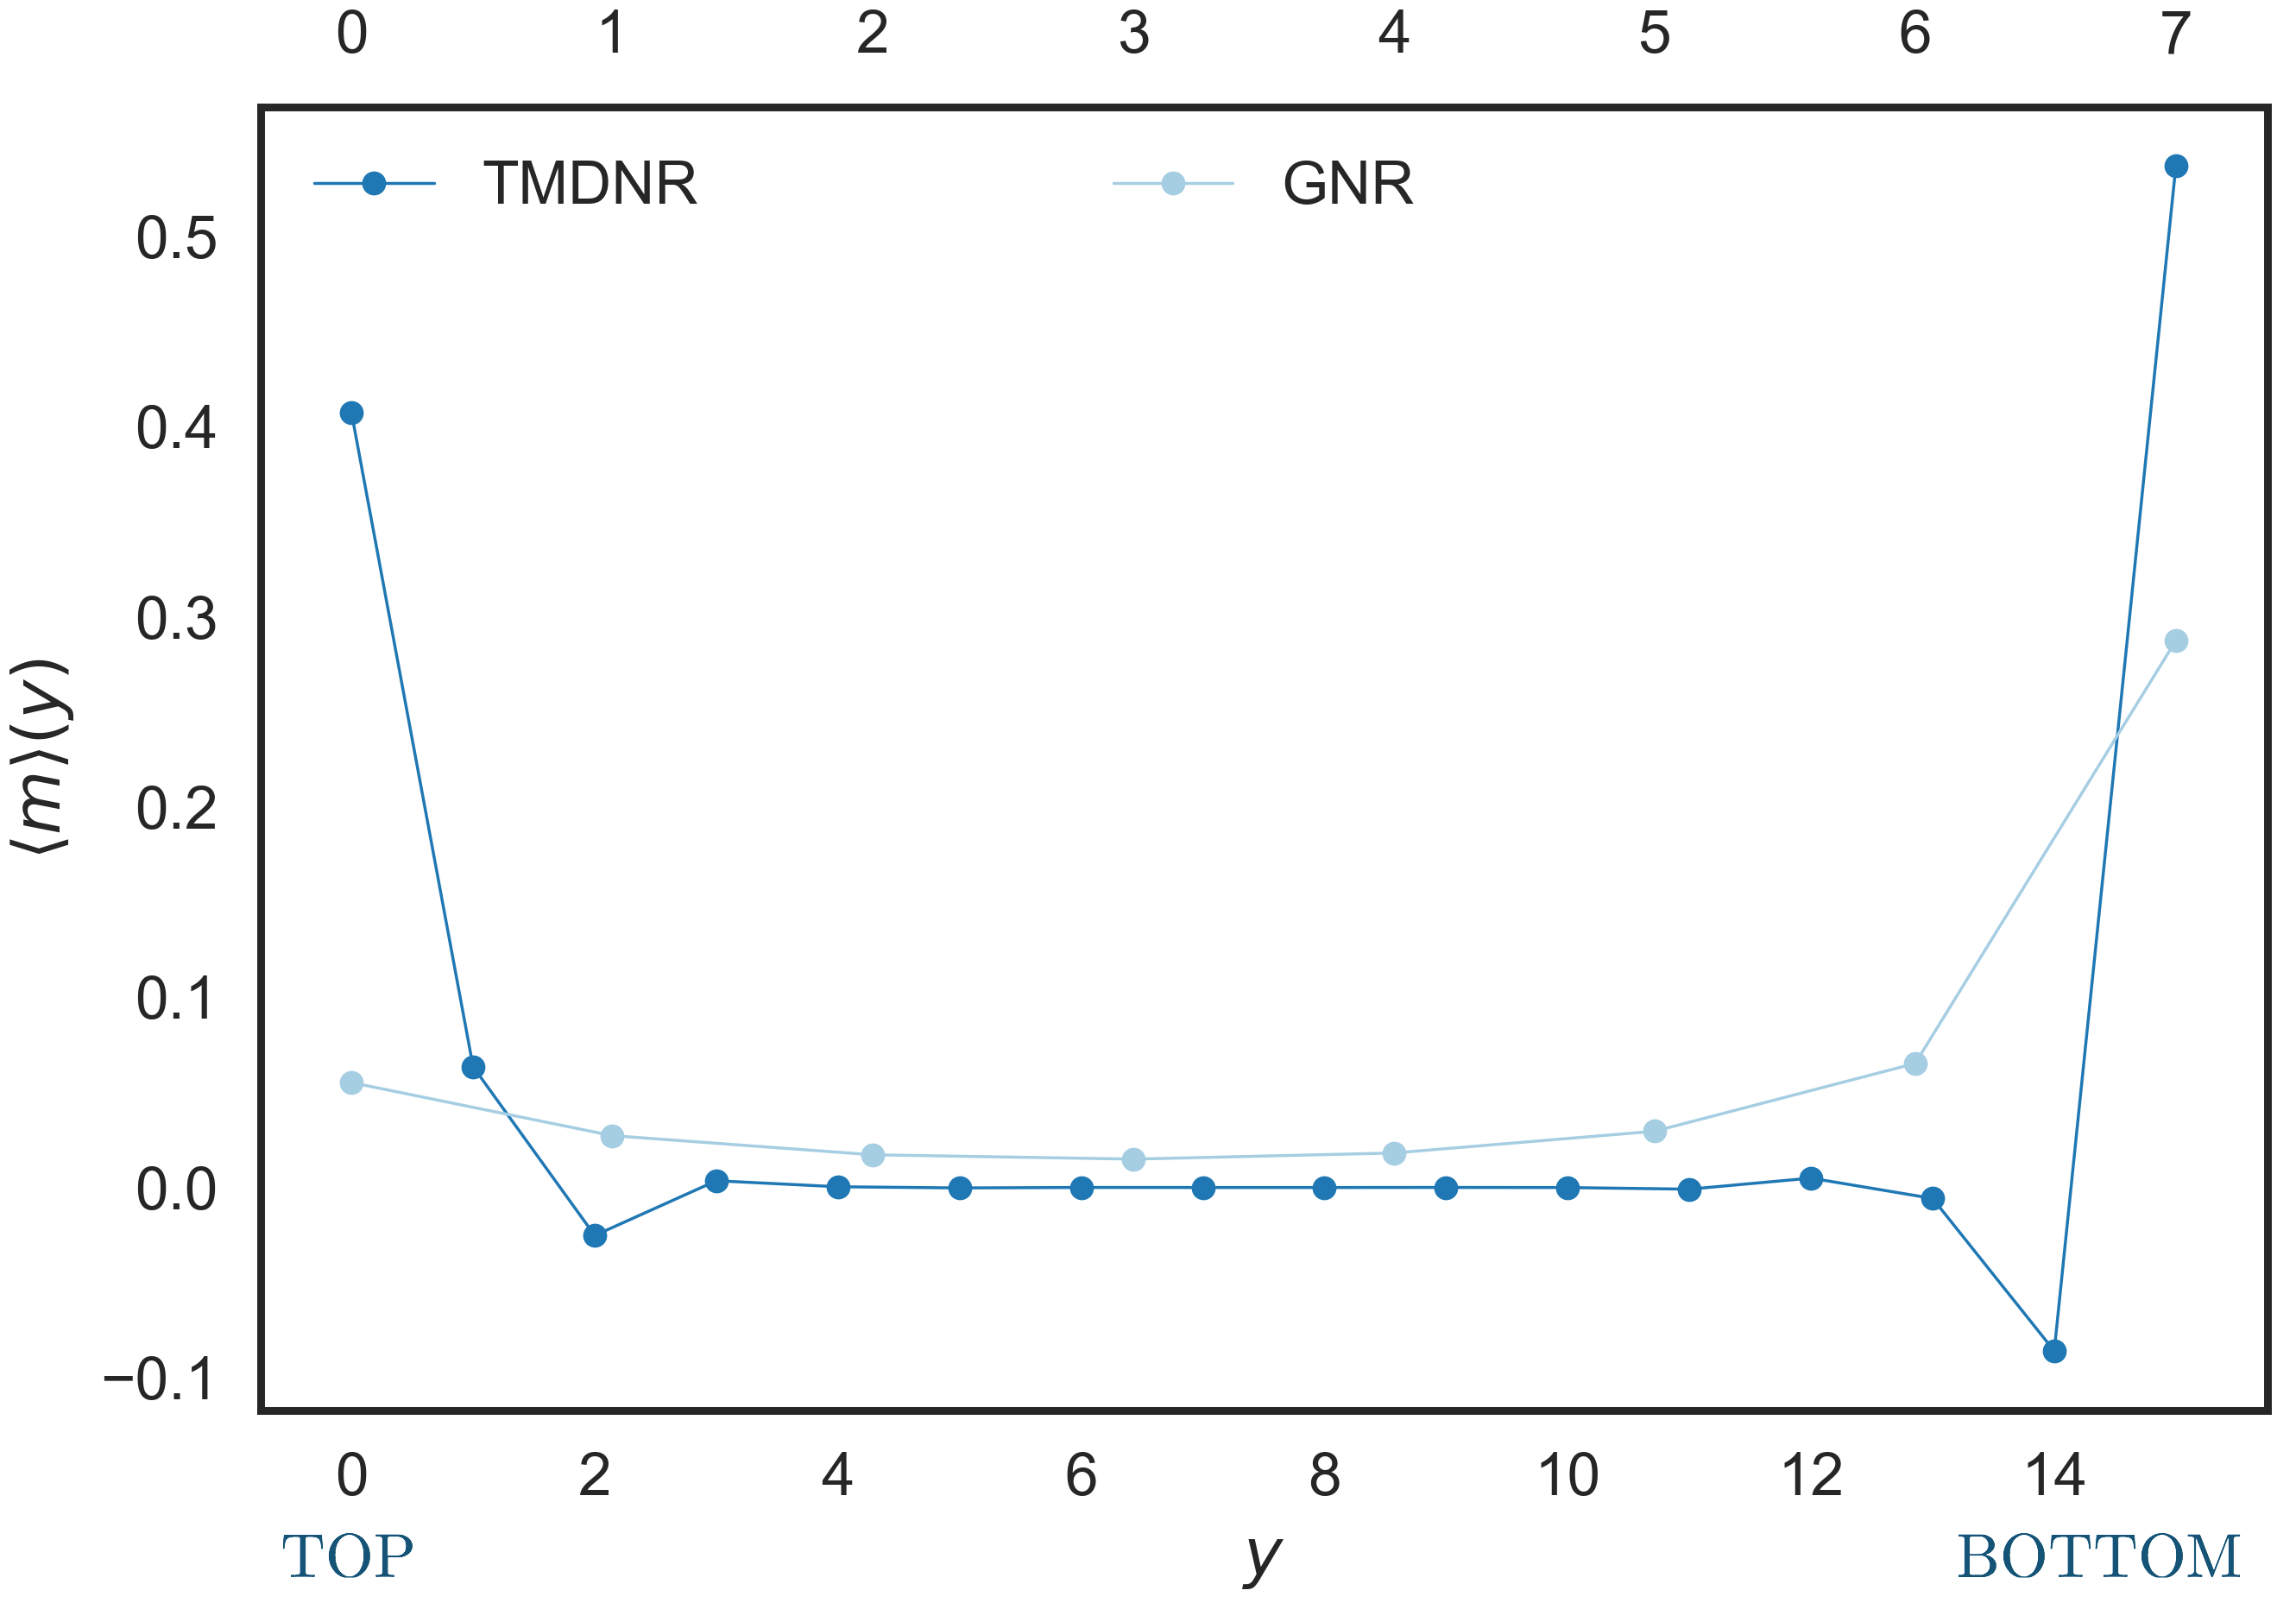
\includegraphics[scale=0.55]{images/magProf.png}
	\caption{Ordered phases.
	Spin density profile along the ribbon's transverse direction $\left\langle m \right\rangle (y)$ for the Hubbard model at half filling ($\left\langle n \right\rangle = 1$) for a $16 \times 8$ graphene nanoribbon (GNR) at $U=1.2t$ (left) and a TMDNR with $N_y = 16$ at $U = 20| t_0 |$, and electron density $\left\langle n \right\rangle = 0.66$, the filling that corresponds to charge neutrality.}
	\label{fig:nanoGraphVsTMD}
\end{figure}
The edge magnetization is due to the different occupation of the spin-up (in red) and spin-down bands (in blue).
As the red, spin-up band near the Fermi energy rests completely below it, its electronic states are all occupied, while the corresponding spin-down states are all above $\varepsilon_F$, and thus are unoccupied.
If these states were extended throughout the sample, a magnetization would appear in the bulk as well.
However, as we show later, the wave functions corresponding to the states near the Fermi energy are heavily localized at the edges.
This means that the spin polarization will be restricted to the edges.
Initially, the up and down states are equally occupied.
As we start increasing $U$, one of the bands (say, the up band) becomes more occupied than the other.
The states in this band correspond only to one of the edges.
Suppose it is the top edge.
As we keep increasing $U$, the band structure changes and eventually, the up band corresponding to the bottom edge becomes occupied than the down spin, bottom edge band, and both edges become magnetized.
\begin{figure}[H]
\centering
    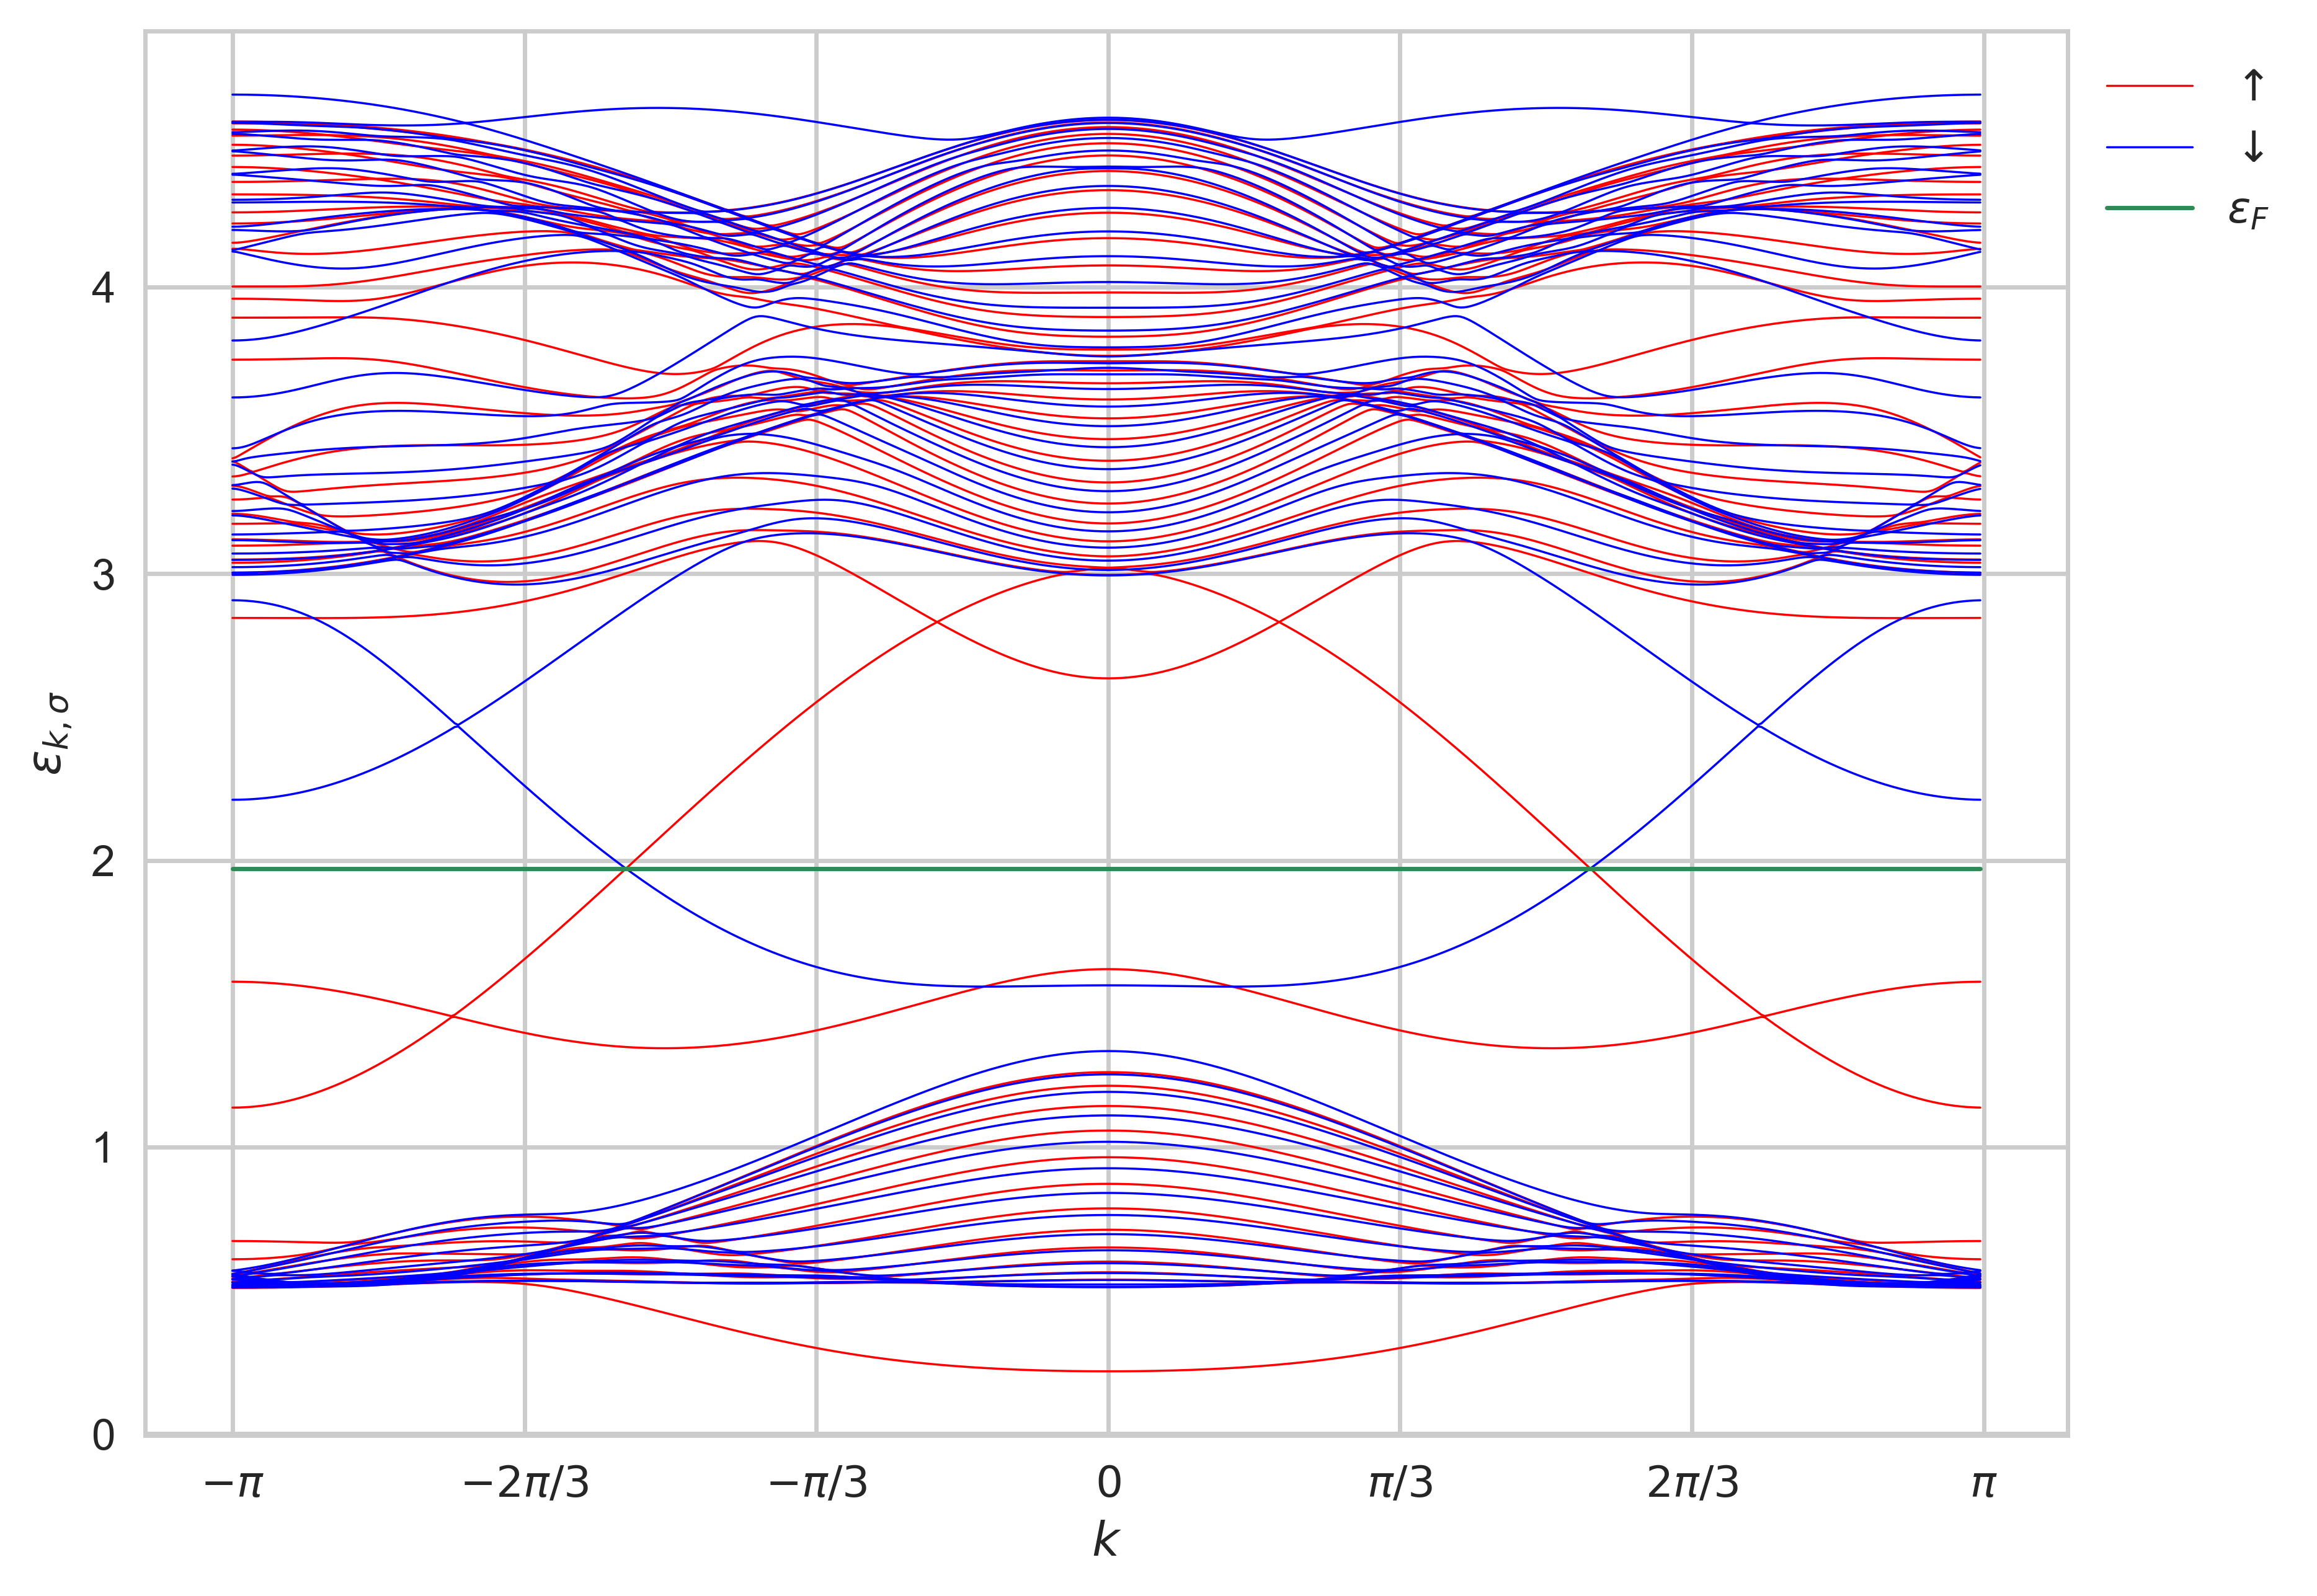
\includegraphics[scale = 0.42]{images/bands_Nx=512.png}
  \caption{Spin-resolved band structure within the ordered phase of a TMD nanoribbon of width $N_y = 16$, at $U = 20$.}
  \label{fig:bandsU20}
\end{figure}
\begin{figure}[H]
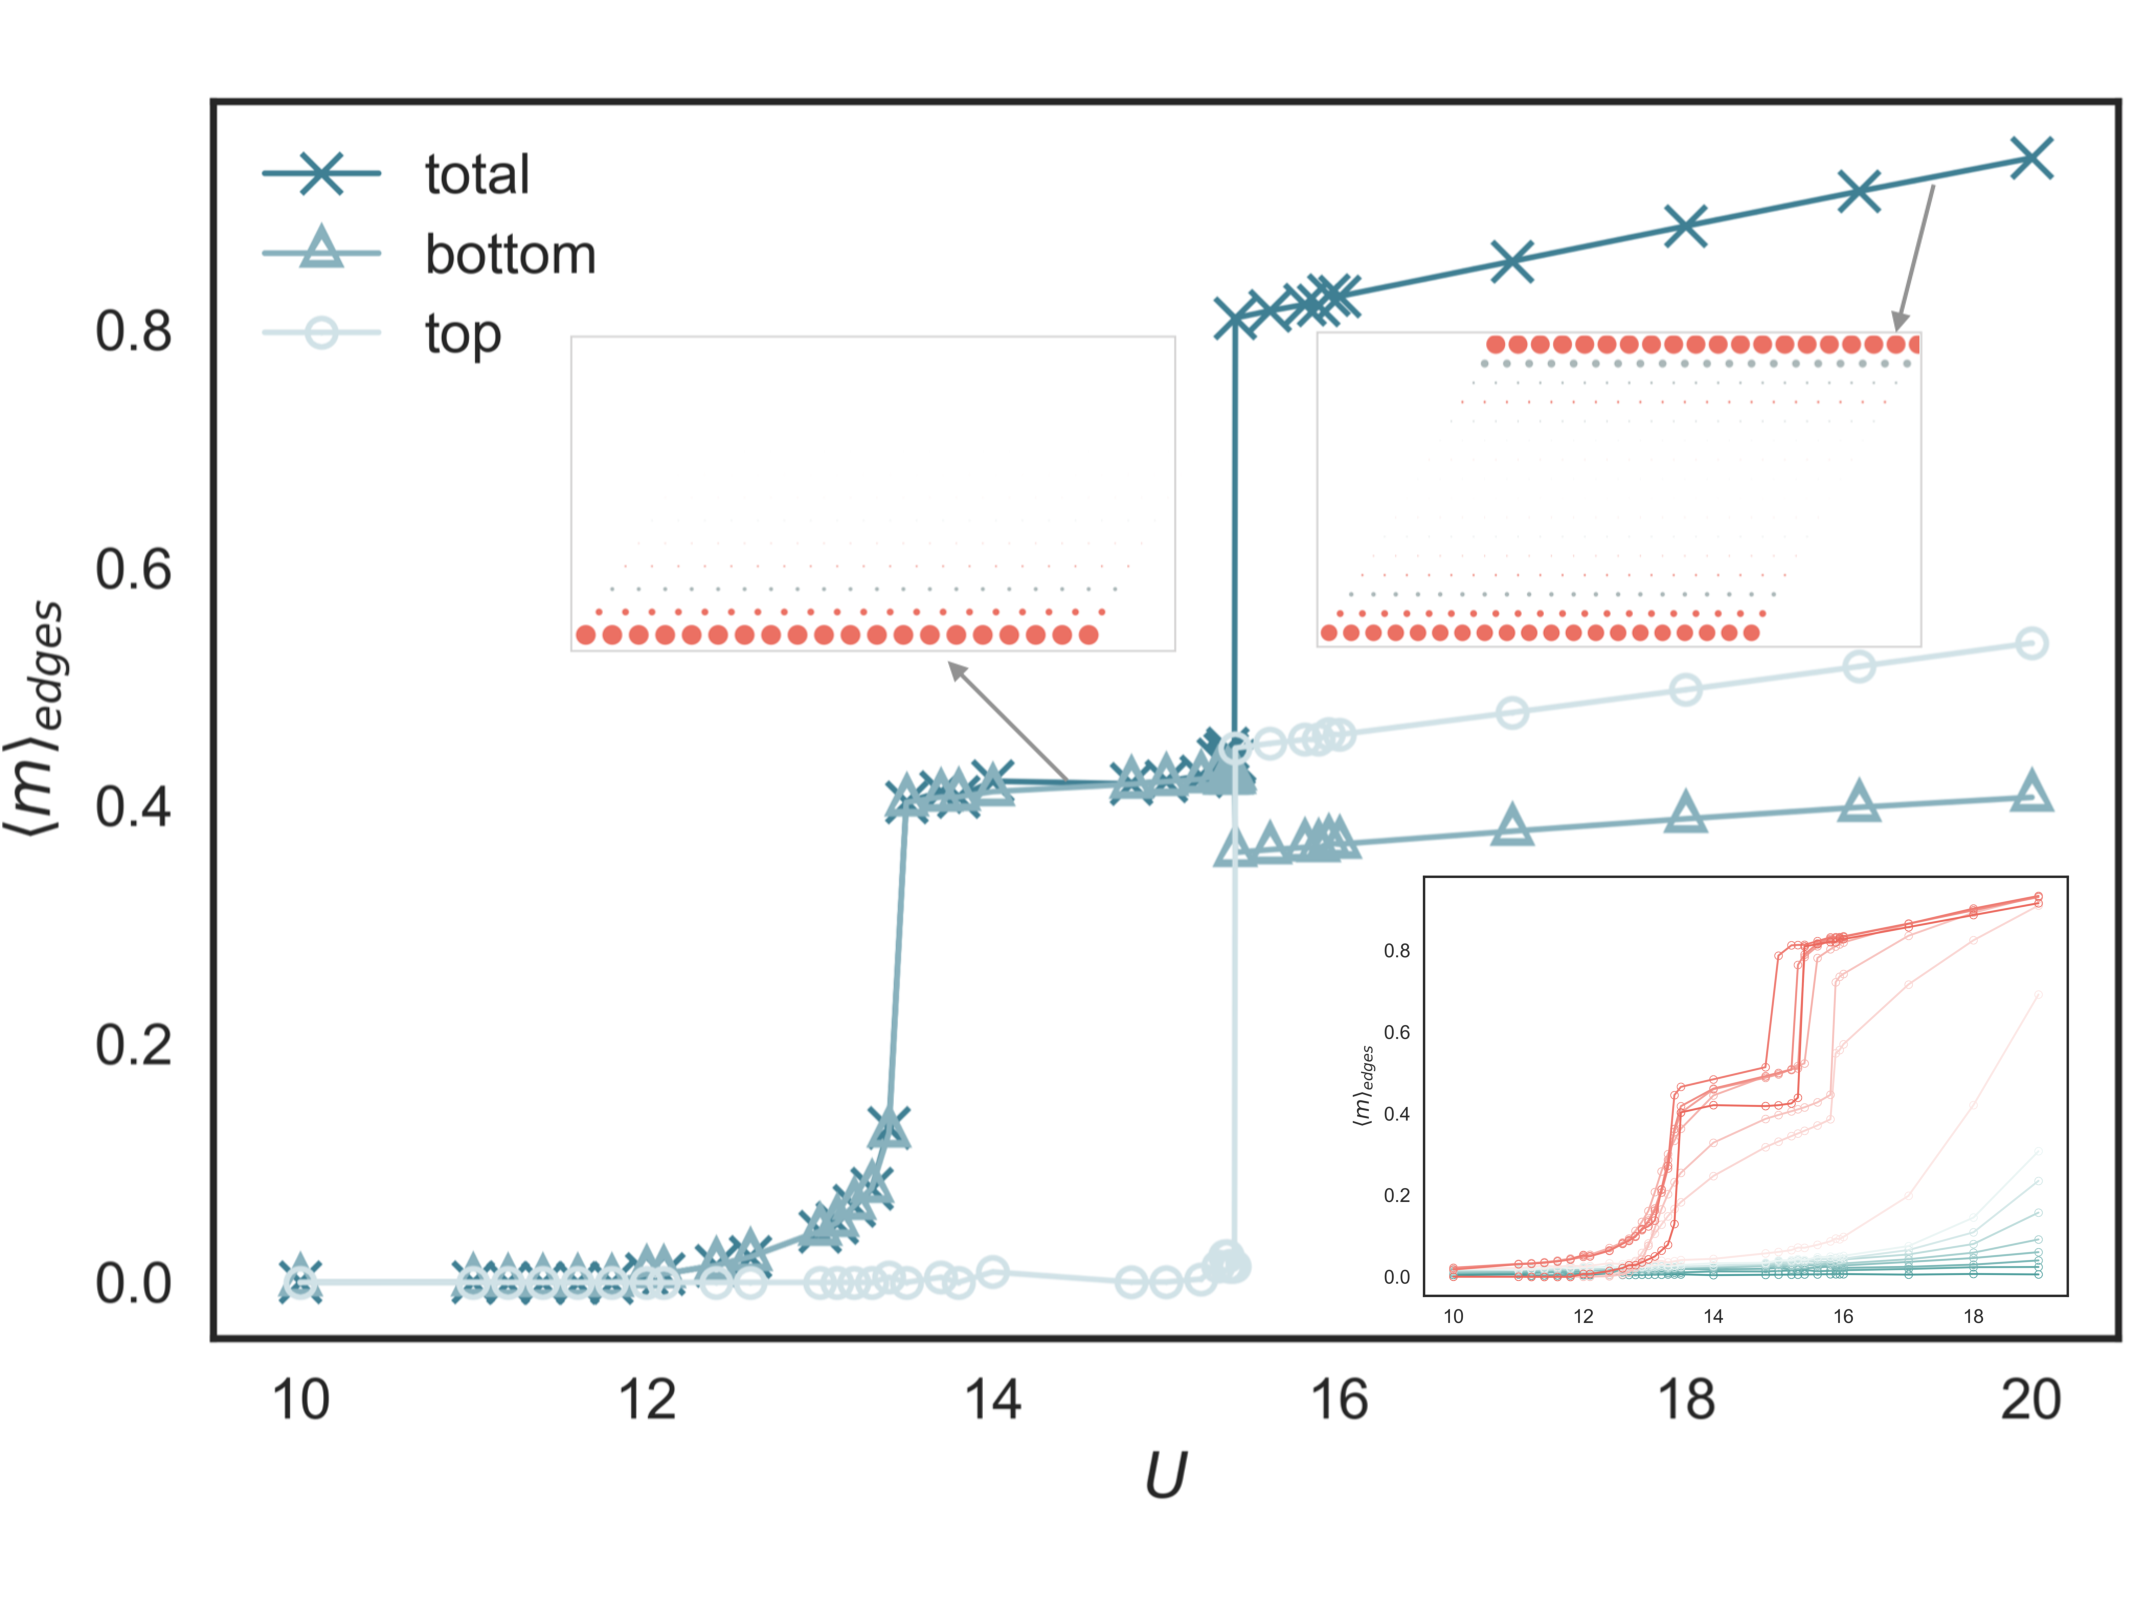
\includegraphics[trim={0cm 1.6cm 0cm 1.6cm},clip, scale =0.21]{images/edgeMagInsetBeta.pdf}
	\caption{Mean field phase diagram at zero temperature and its change as temperature is increased (inset). We analyze the diagram in the inset in the thesis.\label{fig:mfPhaseDiag0}}
\end{figure}
In Fig.(\ref{fig:mfPhaseDiag0}), we show the zero temperature phase diagram of a a TMD nanoribbon of width $N_y = 16$, and $\left\langle n \right\rangle = 0.66$ (we use this filling throughout).
By solving the self-consistent equation iteratively, at zero temperature, for varying $U$, we find two phase transitions, with respective critical on-site interactions $U_{c_1} \approx 11.8 |t_0|$, and $U_{c_2} \approx 15.395 |t_0|$.
The second phase transition is much more abrupt than the first transition.
The latter, at $U_{c_1} \approx 11.8 |t_0|$,  appears to be continuous, while the former,  at $U_{c_2} \approx 15.395 |t_0|$ appears to be first order.
%\begin{figure}[H]
%\centering
%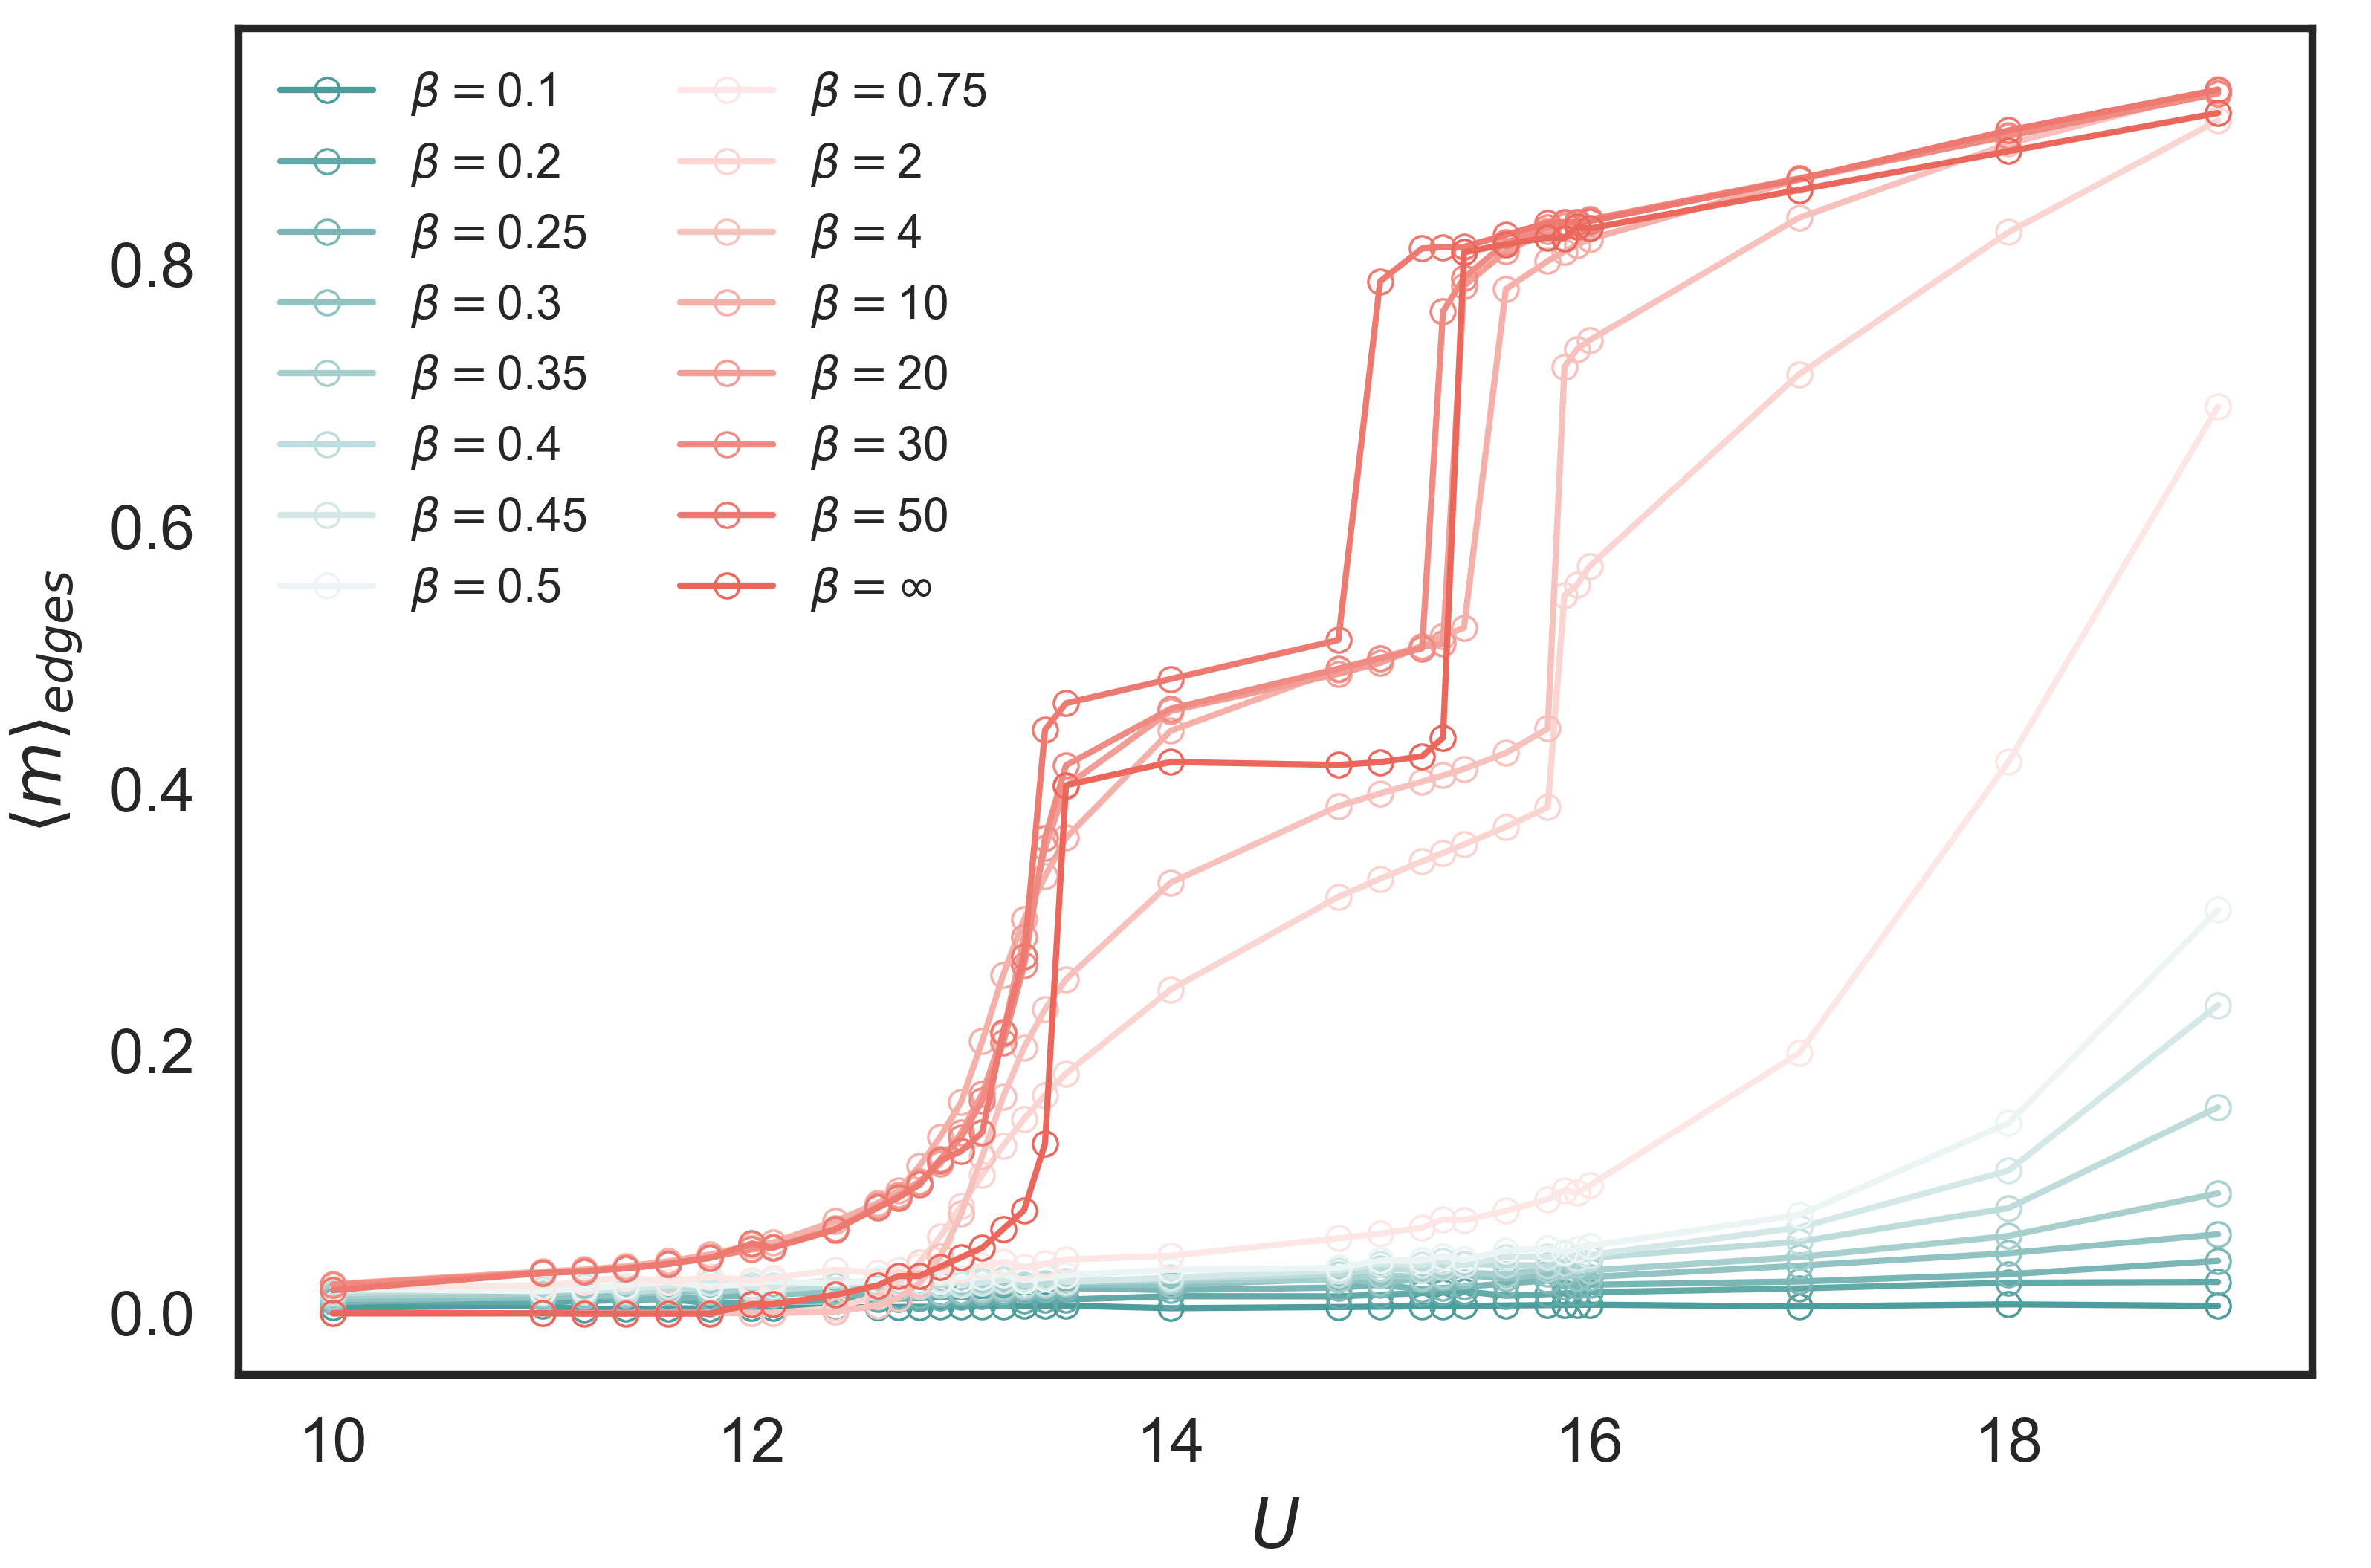
\includegraphics[width = 7.5cm]{images/edge-mag-phase-diagram.png}
%	\caption[$T=0$ mean field band structure for a TMD nanoribbon of width $N_y = 16$ in the ordered phase, at $U=20 | t_0 |$.]{$T=0$ mean field band structure for a TMD nanoribbon of width $N_y = 16$ in the ordered phase ($U=20 | t_0 |$).\label{fig:mfPhaseDiagT}.}
%\end{figure}
Fig.(\ref{topEdge}) shows the electronic edge states for the different orbitals obtained in our mean field calculation.
This diagram corresponds to the phase at $U=13$ at zero temperature.
We see that as the shown spin-up states localized at the top edge have become occupied (with respect to the disordered phase) and their corresponding spin-down states unoccupied, a magnetization sets in.
\begin{figure}[H]
  \centering
  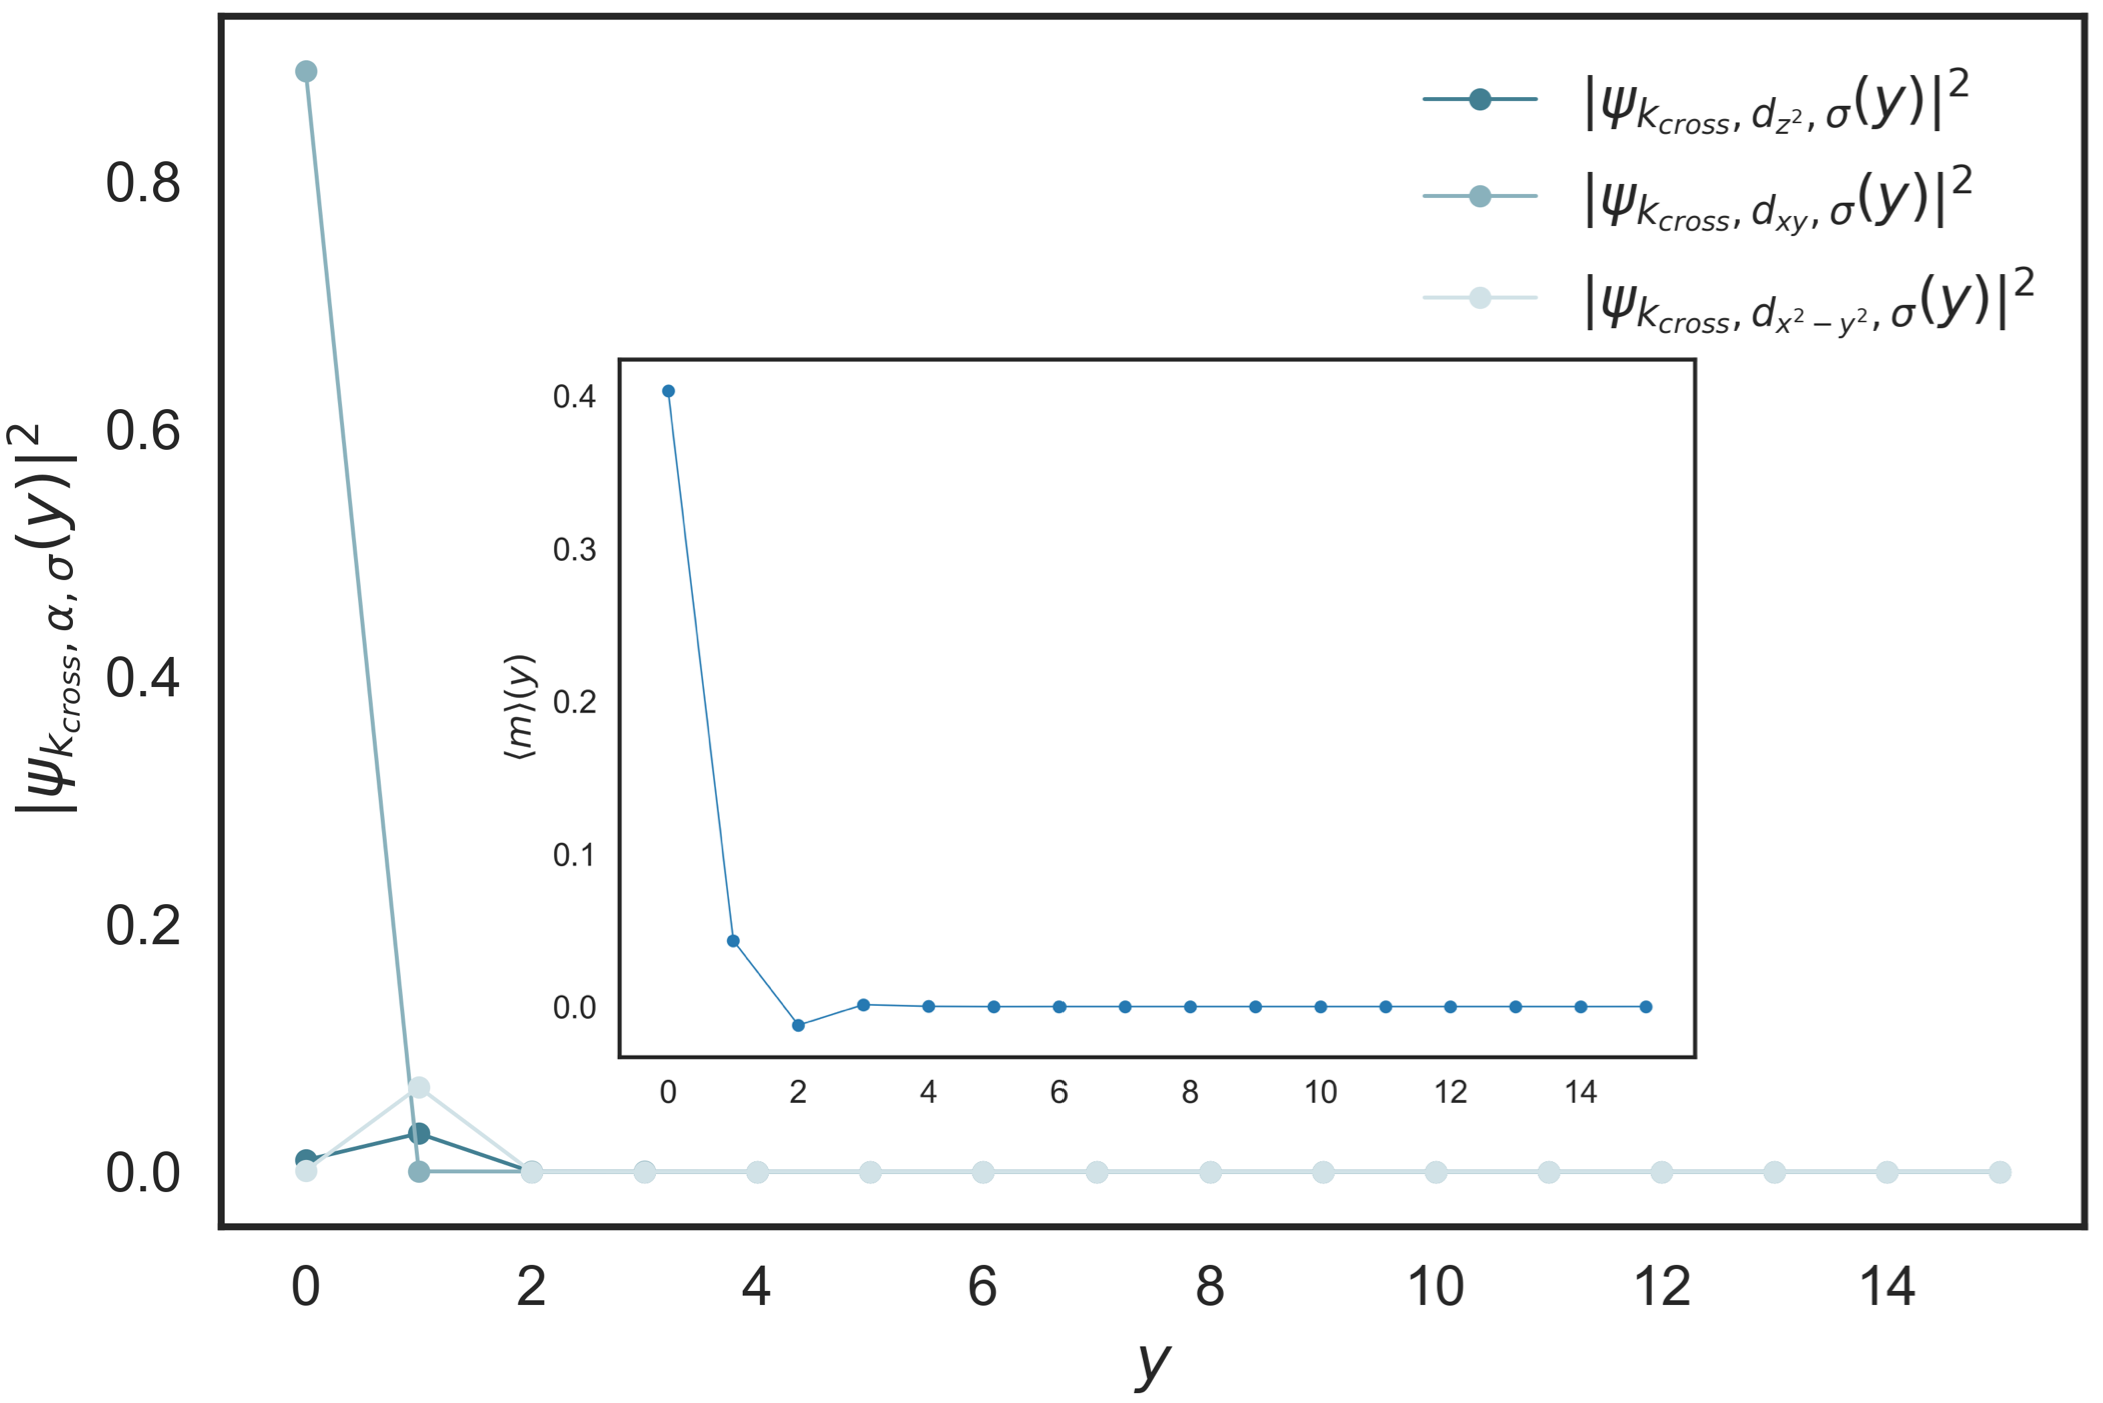
\includegraphics[width=7.3cm]{images/topEdgeMagProfU13.png}
  \caption{Localized edge states on the top of the ribbon, at $U = 13 |t_0|$ for the different orbitals. Inset: Resulting magnetization profile along the ribbon's transverse direction due to higher spin up than spin down occupation of these states, showing, respectively top edge magnetization.}
  \label{topEdge}
\end{figure}
\begin{figure}[H]
  \centering
  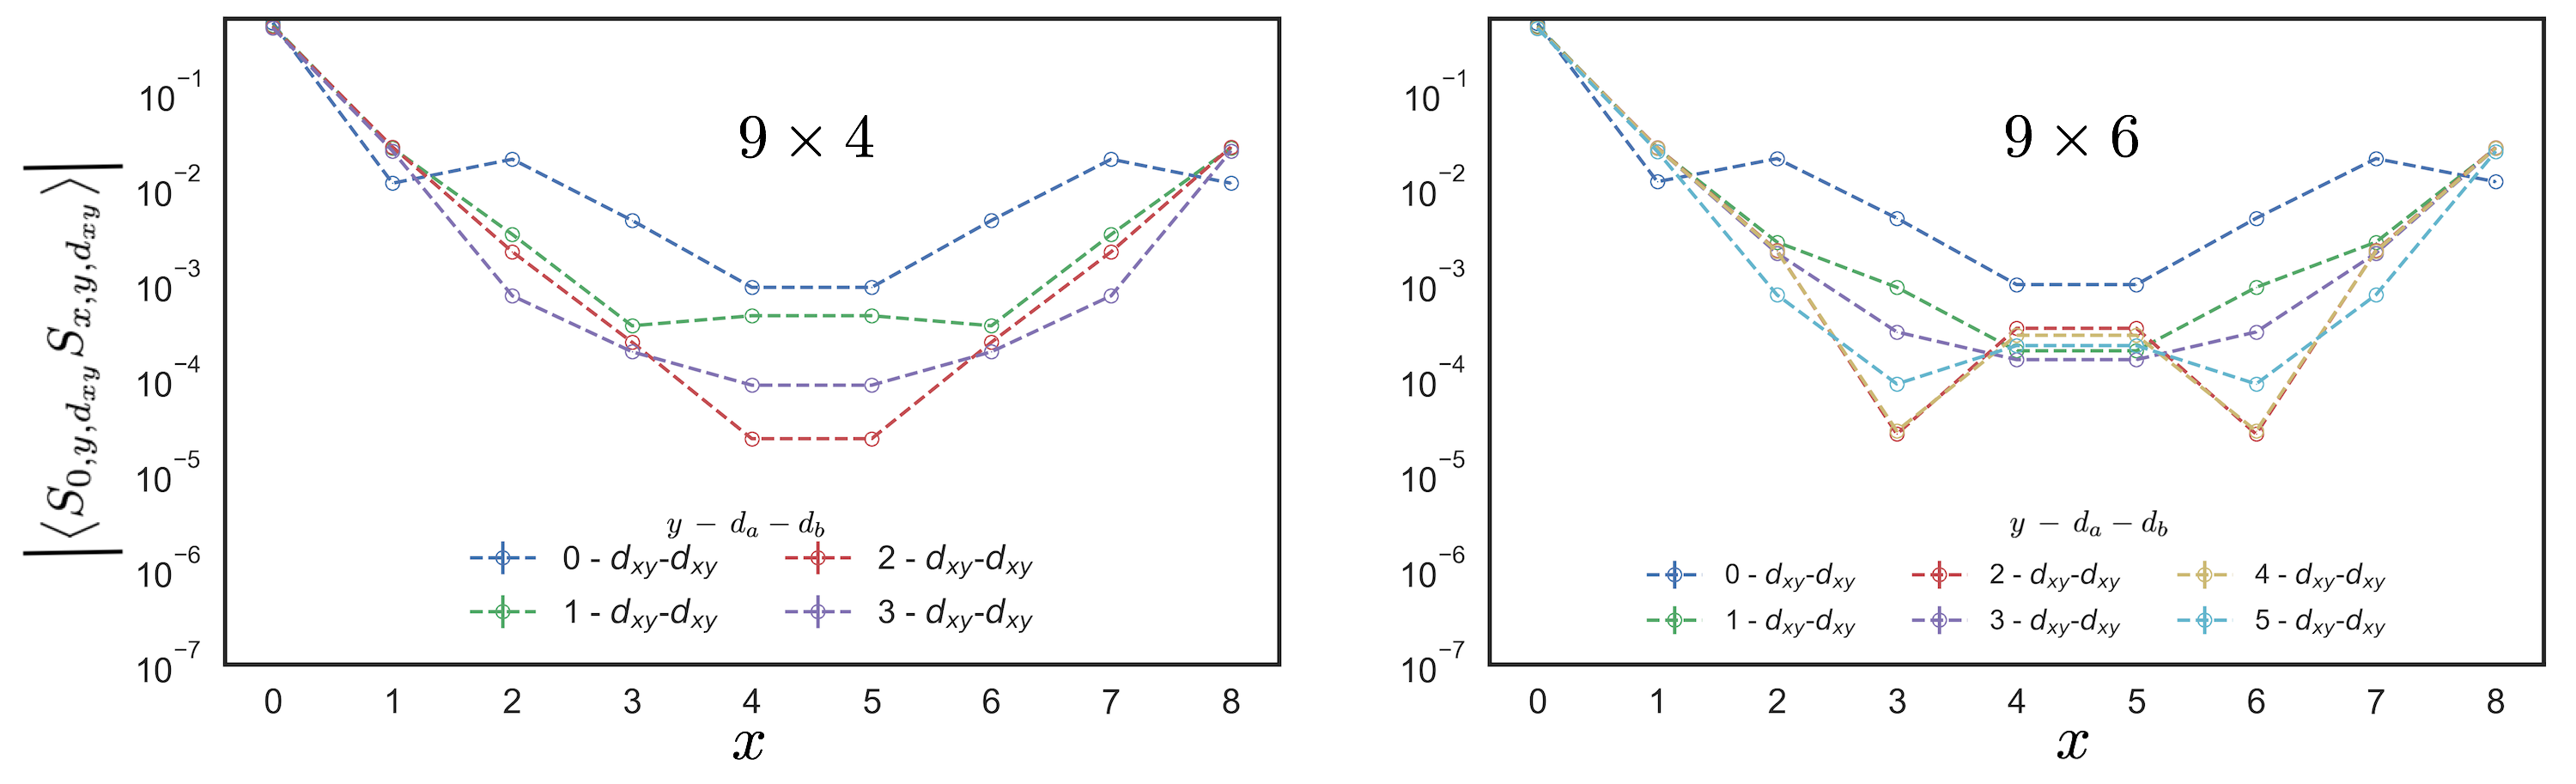
\includegraphics[width=7.3cm]{images/tmdFinalxyxy.png} \\
    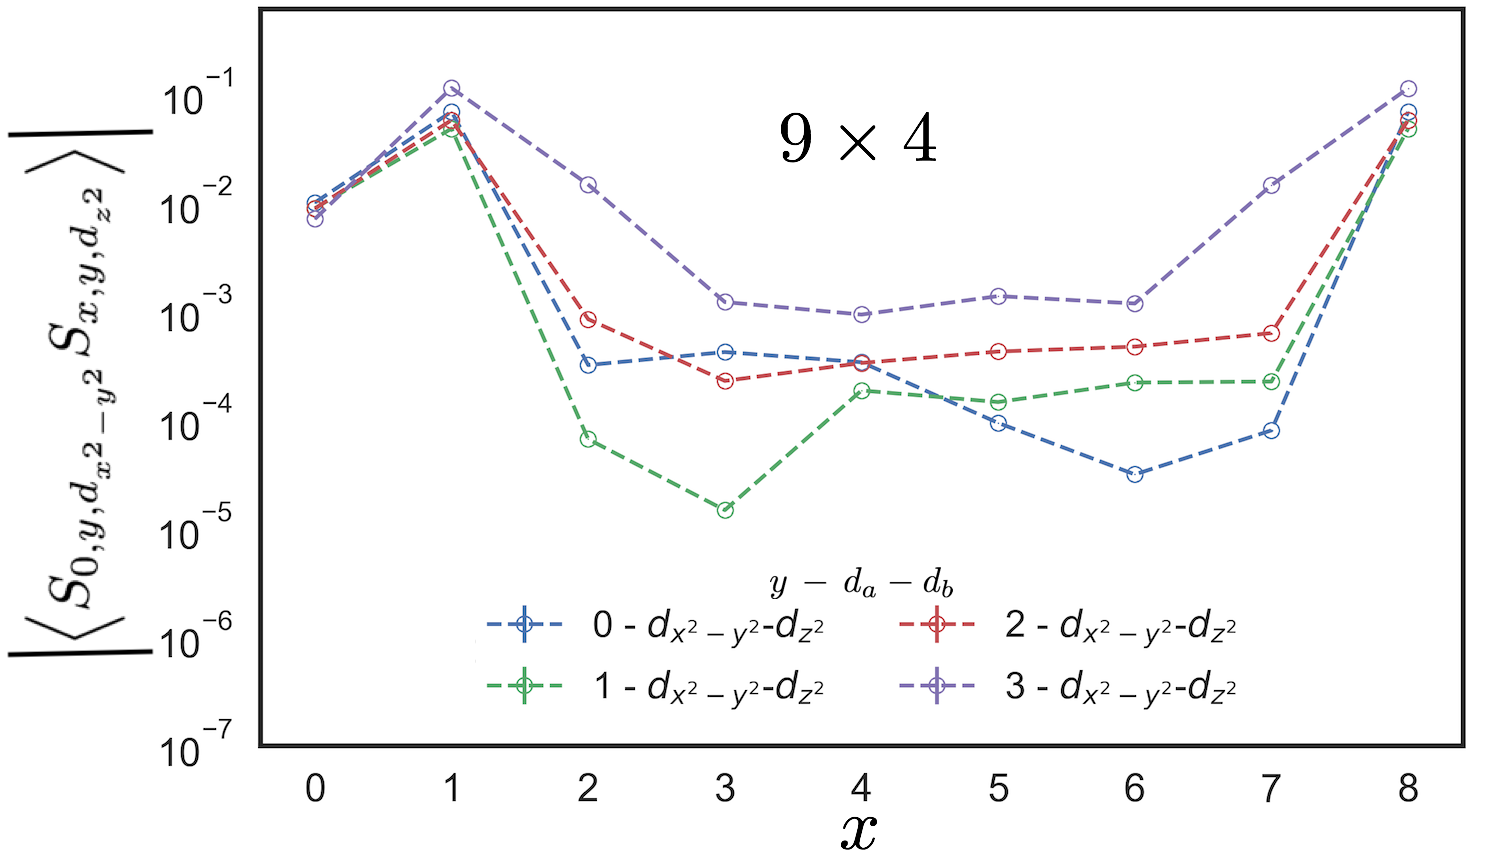
\includegraphics[width=7.3cm]{images/tmdFinalx2y2z2.png}
  \caption{Longitudinal profile (along the $x$ direction) of some of the orbital-resolved $S^z$ spin-spin correlation functions for two lattice sizes $9 \times 4$ and $9 \times 6$ ($d_{x^2-y^2} d_{z^2}$ and $d_{xy} - d_{xy}$).
	We use translational invariance along the $x$ direction to average these correlations to improve the statistical properties of the estimator.
	On the left, curves 0, and 3 show correlations along the edge rows, while on the right, curves 0 and 5 correspond to the edges.}
  \label{fig:corrQMC}
\end{figure}
In Fig.(\ref{fig:corrQMC}), we show an example of a result of our QMC code for a TMD nanoribbon.
In the model we consider, the sign problem severely restricts the range of parameters $U$, $\beta$, $\mu$ (or $\left\langle n \right\rangle$) that we can explore.
In fact, for $\beta > 2 | t_0 |$, the average sign rapidly goes to zero for the range of on-site interactions where mean field predicts the existence of an ordered phase.
Nonetheless, for the considered sizes, at $\beta = 2 | t_0 |$ and $U = 16$, and at the relevant electron density $\left\langle n \right\rangle = 0.66$, the sign problem is not prohibitive ($\left\langle \text{sign} \right\rangle \sim0.4$).
Fig.(\ref{fig:corrQMC}) indicate that the complexity of the problem is much higher than, for example, in the case of graphene.
Furthermore, recent analogous studies for graphene \cite{feldner_dynamical_2011, yang_strain-tuning_2017,raczkowski_interplay_2017} suggest that one needs thicker ribbons to measure long range ordering with enough accuracy, which implies taking larger system sizes.
To be conclusive about the true nature of edge-magnetism in TMDNRs, given the increased complexity of our model, this requires an enormous amount of computer time (about 20 times, or possibly more than for the analogous graphene studies), which we shall have access to very soon.
%%%%%%%%%%%%%%%%%%%%%%%%%%%%%%%%%%%%%%%%%%%%%%%%%%%%%%%%%%%%%%%%%%%%%%



